\chapter{Corrispondenze e relazioni di equivalenza}

\section{Corrispondenze e relazioni binarie}

\begin{defbox}{Corrispondenza}\index{Corrispondenza}
	Dati due insiemi $a$, $b$, una \textbf{corrispondenza} da $a$ a $b$ è una terna ordinata:
	\begin{equation}
		\rho = (a,b,G)
	\end{equation}
	tale che: $G \subseteq a \times b$. L'insieme $G$ prende il nome di \textbf{grafico}\index{Grafico} della corrispondenza $\rho$.
\end{defbox}

Per ogni $x \in a$ e per ogni $y \in b$ scriveremo: $x \; \rho \; y  \iff (x,y) \in G$ per dire che gli elementi $x$ e $y$ sono in \textit{corrispondenza} mediante $\rho$. In questo caso si dice che $y$ è il \textbf{corrispondente}\index{Corrispondente} di $x$ (non il contrario!). La coppia ordinata $(x,y)$ appartiene quindi al grafico $G$. Con il simbolo $Corr(a,b)$ si denota l'insieme di tutte le corrispondenze tra $a$ e $b$: 
\begin{equation}
	Corr(a,b) = \{(a,b,G) \; | \; G \subseteq a \times b \}
\end{equation}

\begin{defbox}{Relazioni binarie}\index{Relazione binaria}\label{def:rel_binaria}
	Una \textbf{relazione binaria} è una corrispondenza tra un insieme $a$ e se stesso. Con il simbolo $Rel(a)$ si denota l'insieme di tutte le relazioni binarie in $a$:
	\begin{equation}
		Rel(a) = Corr(a,a)
	\end{equation}
\end{defbox}

\begin{defbox}{Diagonale}\index{Diagonale}
	Sia $a$ un insieme. L'insieme:
	\begin{equation}
		\Delta_{a}=\{(x,x)\;|\;x \in a\}\subset a \times a
	\end{equation}
	prende il nome di \textbf{diagonale} di $a$ e lo si indica col simbolo $\Delta_{a}$.
\end{defbox}


\begin{example}
	Si consideri l'insieme $A=\{0,1,2,3,4\}$, la diagonale $\Delta_{A}$ è rappresentata dall'area gialla evidenziata di seguito:
	\begin{center}
		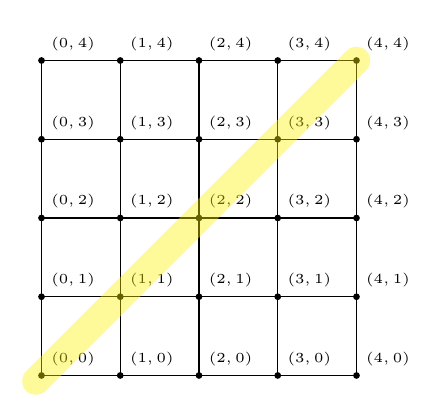
\begin{tikzpicture}
			[strip/.style = {
				draw=#1,
				line width=1em, opacity=0.4,
				line cap=round ,
			}]
			\draw[step=1.0,black,thin] (0,0) grid (4,4);
			\foreach \x in {0,...,4}
			\foreach \y in {0,...,4}
			\filldraw (\x,\y) circle[radius=1pt] node[above right] {\tiny $(\x,\y)$};
			\path[draw,strip=yellow,shorten <=-1mm] (0,0) -- (4,4);
		\end{tikzpicture}
	\end{center}
\end{example}

\begin{example}
	Tra le relazioni binarie in un insieme $s$ vi sono la \textbf{relazione identica} $\iota_{s} = (s,s, \Delta_{s})$ e la \textbf{relazione totale} $\tau_{s}=(s,s,s \times s)$. È chiaro che nella relazione identica ogni elemento è in relazione soltanto con se stesso mentre nella relazione totale ogni elemento di $s$ è in relazione con ciascun elemento.
\end{example}

\subsection{Proprietà delle relazioni binarie}
\begin{defbox}{Relazione opposta}\index{Relazione opposta}
	Sia $\rho = (s,s,G)$ una relazione binaria nell'insieme non vuoto $s$ e si ponga $G^{*}=\{(y,x)\;|\; (x,y) \in G\}$. Allora la coppia $\rho^{*}=(s,s,G^{*})$ è una relazione binaria in $s$ che prende il nome di \textbf{relazione opposta} di $\rho$.
\end{defbox}

Sia $s$ un insieme non vuoto. Per una relazione binaria $\rho = (s,s,G)$ in $s$ si danno le seguenti definizioni:
\begin{itemize}
	\item $\rho$ si dice \textbf{riflessiva} se	$\forall x \in s (x \ \rho \ x)$, cioè se il grafico $G$ contiene la diagonale $\Delta_{s}$;
	\item $\rho$ si dice \textbf{antiriflessiva} se $\forall x \in s \; (x \ \cancel{\rho} \ x)$, cioè se il grafico $G$ è disgiunto dalla diagonale $\Delta_{s}$;
	\item $\rho$ si dice \textbf{simmetrica} se per ogni coppia $(x,y)$ di elementi di $s$ tali che $x \ \rho \ y$ si ha anche $y \ \rho \ x$, cioè se $\rho$ coincide con la sua relazione opposta $\rho^{*}$.
	\item $\rho$ si dice \textbf{asimmetrica} se da $x \  \rho  \ y$ e $y \rho x$ segue $x=y$.
	\item $\rho$ si dice \textbf{transitiva} se qualunque siano gli elementi $x$, $y$ e $z$ di $s$ tali che $x \ \rho \ y$ e $y \ \rho \ z$, si ha anche $x \ \rho \ z$.
\end{itemize}

\subsection{Rappresentazione delle corrispondenze}

\begin{example}
	Dati $A=\{0,1,2\}$ e $b=\{0,4\}$ si avrà che l'insieme $A \times b$ conterrà le coppie ordinate:
	\begin{displaymath}
		A \times b = \{(0,0),(0,4),(1,0),(1,4),(2,0),(2,4)\}
	\end{displaymath}
	Dunque esisteranno $2^{6}=64$ sottoinsiemi del prodotto cartesiano, ovvero 64 diverse tipologie di corrispondenze tra gli insiemi $A$ e $b$. Per descrivere dunque una corrispondenza può essere comodo esprimere la \textbf{condizione di appartenenza} al grafico della corrispondenza. Ad esempio il grafico:	$G = \{(x,y) \in A \times b \; | \; x < y \}$ esprime l'insieme:
	\begin{displaymath}
		G = \{(0,4),(1,4),(2,4)\} \subset A \times b
	\end{displaymath}
	Che descrive la seguente definizione di corrispondenza:
	\begin{displaymath}
		\alpha \in Corr(A,b) \qquad \mbox{definito da} \quad \forall x \in A \; \forall y \in b \quad \bigl( x \; \alpha \; y \iff x <y \bigr)
	\end{displaymath}
\end{example}

\begin{example}
	Oltre a rappresentare una corrispondenza mediante il proprio grafico è possibile utilizzare anche una rappresentazione grafica mediante i diagrammi di Venn oppure mediante tabelle. Si considerino gli insiemi $A=\{1,2,3\}$, $b=\{x,y\}$ e la corrispondenza $\rho=(A,b,\{(1,x),(1,y),(3,y)\})$. Si hanno quindi le seguenti rappresentazioni:
	\begin{center}
		\begin{minipage}{.45\textwidth}
			\centering
			\begin{tikzpicture}
				\filldraw[black] (0,0) circle (2pt) node[anchor=west] (1) {$1$};
				\filldraw[black] (0,-1) circle (2pt) node[anchor=west] (2) {$2$};
				\filldraw[black] (0,-2) circle (2pt) node[anchor=west] (3) {$3$};
				\filldraw[black] (4,-1) circle (2pt) node[anchor=west] (4) {$x$};
				\filldraw[black] (4,-2) circle (2pt) node[anchor=west] (5) {$y$};
				\node[shape=ellipse,minimum width=2cm,draw=blue,fit={(1)(2)(3)},,label=above:$A$](e3){};
				\node[shape=ellipse,minimum width=2cm,draw=green,fit={(4)(5)},label=above:$b$]{};
				\draw[->,xshift=-5pt](1)to[bend left=25](4,-1);
				\draw[->,xshift=-5pt](1) to [bend right=25](4,-2);
				\draw[->,xshift=-5pt](3) to [bend right =25] (4,-2);
			\end{tikzpicture}
			\captionof{figure}{Diagrammi di Venn}
		\end{minipage}
		\hfil
		\begin{minipage}{.45\textwidth}
			\centering
			\begin{tblr}
				{
					hline{1-Z} = {0.9pt},
					vline{1-Z} = {0.9pt},
					vline{1} = {1}{0pt},
					hline{1} = {1}{0pt},
					cell{1}{2-Z}={primary!40!white},
					cell{2-Z}{1}={primary!40!white}
				}
				& $x$ & $y$ \\
				1 & $\bullet$ & $\bullet$ \\
				2 & & \\
				3 & & $\bullet$
			\end{tblr}
			\captionof{table}{Rappresentazione tabellare}
		\end{minipage}
	\end{center}
\end{example}

\subsection{Prodotto relazionale}\label{prodotto_relazionale}

\begin{defbox}{Prodotto relazionale}
	Siano $A,B,C$ insiemi e $\varphi \in Corr(A,B)$, e $\psi \in Corr(B,C)$ corrispondenze. Il \textbf{prodotto relazionale} di $\varphi$ per $\psi$, denotata con $\varphi \psi$, è la corrispondenza definita ponendo:
	\begin{equation}
		\forall a \in A, \forall c \in C \qquad a \ \varphi \psi \ c \iff \Bigl( \exists b \in B \bigl( (a \ \varphi \ b) \wedge (b \ \psi \ c)\bigr)\Bigr)
	\end{equation}
	
\end{defbox}

\begin{teorbox}[Associatività del prodotto relazionale]
	Il prodotto relazionale gode della proprietà associativa, cioè se:
	$\alpha \in Corr(A, B), \ \beta \in Corr(B,C), \ \gamma \in Corr(C,D)$	sono corrispondenze, allora vale:
	\begin{equation}
		(\alpha \beta) \gamma = \alpha(\beta \gamma)
	\end{equation}
\end{teorbox}

\begin{proof}
	Deve essere, per ogni $a \in A$ e per ogni $d \in D$:
	\begin{align*}
		a \ (\alpha \beta) \ \gamma d & \iff \exists c \in C \bigl( a \ \alpha \beta \ c \wedge c \ \gamma \ d \bigr)  \\
		& \iff \exists c \in C \bigl( \exists b \in B (a \ \alpha \ b \wedge b \ \beta \ c) \wedge c \ \gamma \ d \bigr) \\
		& \iff \exists c \in C, \exists b \in B \bigl(a \ \alpha \ b \wedge b \ \beta \ c \wedge c \ \gamma \ d\bigr)
	\end{align*}
	Analogamente:
	\begin{align*}
		a \ \alpha (\beta \gamma) \ d & \iff \exists b \in B \bigl(a \ \alpha \ b \wedge b \ \beta\gamma \ d \bigr)\\
		& \iff \exists b \in B \Bigl( a \ \alpha \ b \wedge \bigl(\exists c \in C (b \ \beta \ c \wedge c \ \gamma \ d) \bigr) \Bigr) \\
		& \iff \exists b \in B, \exists c \in C \bigl( a \ \alpha \ b \wedge b \ \beta \ c \wedge c \ \gamma \ d \bigr)
	\end{align*}
	Dato che le due condizioni sono equivalenti quindi le due corrispondenze coincidono.
\end{proof}

Per ogni insieme $A,B$ e per ogni corrispondenza $\alpha \in Corr(A,B)$ è possibile considerare i prodotti $id_{A}\alpha$ e $\alpha id_{B}$: $$A \stackrel{id_{A}}{\longrightarrow} A \stackrel{\alpha}{\longrightarrow} B \stackrel{id_{B}}{\longrightarrow} B$$E vale: $id_{A}\alpha = \alpha = \alpha id_{B}$. Infatti:
\begin{displaymath}
	x \ \alpha \ b  \implies \bigl( x \ id_{A} \ x \wedge x \ \alpha \ b \bigr) \implies x \ (id_{A} \alpha) \ b
\end{displaymath}
e:
\begin{displaymath}
	x \ (id_{A} \alpha) \ b \implies  \exists y \in A \Bigl( x \ id_{A} \ y \wedge y \ \alpha \ b \Bigr) \implies x \ \alpha \ b
\end{displaymath}
Analogamente, per ogni $x \in A$ e $b \in B$:
\begin{displaymath}
	x \ \alpha \ b \implies \Bigl( x \ \alpha \ b \wedge b \ id_{B} \ b\Bigr) \implies x \ \alpha id_{B} \ b
\end{displaymath}
e
\begin{displaymath}
	x \ \alpha id_{B} \ b \implies \exists c \in B \Bigl( x \ \alpha \ c \wedge c \ id_{B} \ b \Bigr) \implies x \ \alpha \ b
\end{displaymath}

\section{Applicazioni}

\begin{defbox}{Applicazione}\index{Applicazione}
	Un'\textbf{applicazione} (o \textit{funzione} o \textit{mappa}) di $A$ in $B$ è una corrispondenza $\varphi \in Corr(A,B)$ con la seguente proprietà:
	\begin{equation}\label{eq:applicazione}
		\forall x \in A \quad ( \exists! \ y \in B (x \ \varphi \ y))
	\end{equation}
\end{defbox}

Per indicare che $\varphi$ è un'applicazione di $A$ in $B$ scriveremo: $\varphi: A \rightarrow B$ oppure $ A \stackrel{\varphi}{\rightarrow} B$. Per indicare che all'elemento $a \in A$ corrisponde l'unico elemento $b \in  B$ scriveremo $\varphi(a)=b$ oppure $\varphi:a \mapsto b$, $b$ è chiamata ``\textbf{immagine} di $a$ mediante $\varphi$''. L'insieme $A$ prende il nome di \textbf{dominio} dell'applicazione mentre l'insieme $B$ viene chiamato \textbf{codominio}.

\begin{example}
	\begin{enumerate}
		\item La $f$ assegni a ogni numero reale il suo quadrato, si abbia cioè, per ogni $x \in \mathbb{R} \bigl(f(x)=x^{2}\bigr)$. Dominio e codominio di $f$ sono i numeri reali.
		\item La $f$ associa ogni nazione la rispettiva capitale. Ora il dominio di $f$ è l'insieme delle nazioni, e il suo codominio l'insieme delle città.
	\end{enumerate}
\end{example}

\begin{defbox}{Mappa}
	L'insieme delle funzioni dall'insieme $A$ all'insieme $B$ viene chiamato \textbf{mappa} e si indica col simbolo: $$Map(A,B)= \{ \varphi \; | \; \varphi: A \rightarrow B \}$$ Altre notazioni possibili sono quella esponenziale: $B^{A}$ oppure $t(A,B)$.
\end{defbox}

\begin{center}
	\begin{tikzpicture}
		\node[shape=ellipse,draw=blue, minimum height=3cm, minimum width=4cm] (a) {$A$};
		\node[shape=ellipse, draw=blue, minimum height=2cm, minimum width=3cm, right=4cm of a] (b) {$B$};
		\draw[->] (a) to node[above,midway]{$f$} (b);
	\end{tikzpicture}
\captionof{figure}{Diagramma di una mappa dall'insieme $A$ all'insieme $B$}
\end{center}

\begin{osservation}
	Definite le funzioni come terne ordinate si avrà, in base alla Proposizione~\ref{prop_terne_ordinate}, che due funzioni $f=(A,B,G_{f})$ e $g=(C,D,G_{g})$ si diranno equivalenti se, e soltanto se, hanno lo stesso dominio ($A=c$), lo stesso codominio ($B=D$) e lo stesso grafico ($G_{f}=G_{g}$).
\end{osservation}

Spesso per assegnare una funzione $ f\colon A \longrightarrow B$ si fornisce una ``legge'' ossia una qualche formula che permette di associare A ciascun elemento del dominio la sua immagine. Si faccia però attenzione al fatto che la funzione è caratterizzata soltanto dal dominio $A$, dal codominio $B$ e dal grafico $G$ e non dalla eventuale “formulazione della legge”. I due esempi seguenti mostrano come una stessa “legge” può definire funzioni diverse e come, d’altra parte, “leggi” diverse possono definire una stessa funzione.

\begin{example}
\begin{enumerate}
	\item La funzione $f\colon \mathbb{Z}\longrightarrow \mathbb {N}$ data da $f(n)=n^2$ e la funzione $g\colon \mathbb {N} \longrightarrow \mathbb {Z}$
	data da $g(n)=n^2$ sono diverse, perché non hanno lo stesso dominio e lo stesso	codominio, ma, oltre a questo, hanno anche proprietà molto diverse. Usando la terminologia che definiremo in seguito, $f$ non è iniettiva, mentre $g$ lo è.

	\item Siano $A=\{0,1,2\}$ ed $f,g: A \longrightarrow \mathbb{R}$ le funzioni definite rispettivamente da $f(x)=x-7$ e $g(x)=x^3-3x^2+3x-7$. Queste funzioni, per quanto espresse mediante ``leggi'' diverse, sono la stessa funzione, ossia $f=g$, poiché hanno lo stesso dominio, lo stesso codominio e lo stesso grafico: $G_{f} = G_{g} = \{(0,-7),(1,-6),(2,-5)\}$.
\end{enumerate}
\end{example}

\subsection{Questione della ``buona posizione'' delle applicazioni}
Solitamente si trovano notazioni del tipo: $x \in A \mapsto y \in B$
per indicare una funzione $t=(A \times b, G)$ dove: $G=\{(x,y) \; | \; x \in A, y \in B \}$ è il grafico della funzione. È importante saper distinguere le varie notazioni, infatti:
\[
\begin{array}{lc}
	\mathbb{N} \rightarrow \mathbb{Z} \qquad \mbox{viene utilizzata per le corrispondenze tra insiemi} \\
	n \mapsto n+1 \quad \mbox{è la notazione per indicare il valore associato all'elemento n}          \\
\end{array}
\]

È possibile trovare anche notazioni più complicate:
$$
s(x,y,z,...) \in A \mapsto t(x,y,z,...) \in B
$$
dove $s(x,y,z,...)$ è una espressione nelle variabili $(x,y,z,...)$. Non è sempre detto, però, che tali notazioni stiano ad indicare delle vere e proprie applicazioni ``ben definite''. Non sempre l'espressione $s(x,y,z,...)$ è \textit{descrittiva di tutti gli elementi del dominio}, così facendo si otterrebbero elementi del dominio che non godono di corrispondente e questo non va bene secondo la definizione di applicazione. Analogamente, $t(x,y,z,..)$ \textit{deve associare uno ed uno solo elemento del codominio}.

\begin{example}
	Analizziamo le corrispondenze rappresentate dai seguenti grafici:
	\begin{center}
		\includegraphics[scale=.55]{res/Corrispondenze_applicazioni.png}
	\end{center}
	La corrispondenza di figura a rappresenta una funzione.
	La corrispondenza di figura b non rappresenta una funzione perché l’elemento $a$ di $A$ è in corrispondenza con due elementi di $B$, il 2 e il 4, quindi non è una corrispondenza univoca. La corrispondenza della figura c rappresenta una funzione. La corrispondenza della figura d non è una funzione perché il dominio non coincide con l’insieme $A$.
\end{example}

\begin{example}
	L'applicazione: $\beta: x \in \mathbb{N} \mapsto x+1 \in \mathbb{Z}$ è ben posta in quanto per ogni elemento $x \in \mathbb{N}$ esiste ed è unico il suo successivo definito in $\mathbb{Z}$.
\end{example}

\begin{example}
	La corrispondenza $\alpha: n \in \mathbb{N} \mapsto n-1 \in \mathbb{N}$ non è un'applicazione. Infatti l'elemento $0 \in \mathbb{N}$ non ammette precedente. Quando verifichiamo la buona posizione di una applicazione dobbiamo verificare che \textbf{tutti} i valori del dominio abbiano un corrispondente del codominio.
\end{example}

\begin{example}
	La notazione $(a,b) \in \mathbb{R}\times \mathbb{R} \mapsto \frac{a}{b} \in \mathbb{R} $
	non descrive una applicazione in quanto tutte le coppie di seconda coordinata nulla non hanno un loro corrispondente.
\end{example}

\begin{example}
	L'applicazione $n \in \mathbb{N} \mapsto n-1 \in \mathbb{Z}$ è un'applicazione dato che l'insieme di arrivo è quello dei numeri interi.
\end{example}

\begin{example}
	La corrispondenza $X \in \mathcal{P}(\mathbb{Z}) \mapsto X \cap \mathbb{N}\in \mathcal{P}(\mathbb{N})$ è un'applicazione. Infatti ogni parte dell'insieme dei numeri interi, se intersecata con l'insieme dei numeri naturali, è una parte dell'insieme $\mathbb{N}$. Al contrario, la corrispondenza $\{x\}\in \mathcal{P}(\mathbb{Z}) \mapsto \{x\}\cap \mathbb{N} \in \mathcal{P}(\mathbb{N})$ non è un'applicazione. Infatti l'espressione $\{x\}\in \mathcal{P}(\mathbb{Z})$ non è \textit{descrittiva} di tutti gli elementi del dominio $\mathcal{P}(\mathbb{Z})$, esistono quindi elementi che non hanno corrispondenti secondo la formula.
\end{example}

\begin{example}
	La relazione:
	$$
	f=(\mathbb{R} \times \mathbb{R},G) \qquad G=\{(x,y) \in \mathbb{R}^{2} \; | \; y^{2}=x \}
	$$
	non è una funzione poiché contraddice la definizione di applicazione in quanto esistono sempre due numeri $y_{1},y_{2}$ tali che $y_{1}^{2}=y_{2}^{2}=x$, ad esempio $(-2)^{2}=2^{2}=4$.
\end{example}

\begin{example}
	$\{a,b\} \in \mathcal{P}(\mathbb{Z}) \mapsto a+b \in \mathbb{Z}$ \textbf{non} è una funzione poiché non tutti gli elementi del dominio hanno una propria immagine.
	Fissato invece, per ogni insieme $A$ e per ogni naturale $k$, l'insieme:
	\begin{equation}
		\mathcal{P}_{k}(A)=\{X \in \mathcal{P}(A) \ | \ |X|=k\}
	\end{equation}
	
	detto l'\textit{insieme delle parti di $A$ di cardinalità $k$}. Possiamo considerare quindi:
	\[
	\begin{array}{lc}
		p: \{a,b\} \in \mathcal{P}_{2}(\mathbb{Z}) \mapsto a+b \in \mathbb{Z} \\
		q: \{a,b\} \in \mathcal{P}_{2}(\mathbb{Z}) \mapsto a-b \in \mathbb{Z}
	\end{array}
	\]
	Mentre $p$ è una applicazione, $q$ non lo è. Infatti elementi uguali di $\mathcal{P}_{2}(\mathbb{Z})$ hanno immagini distinte: ad esempio l'insieme $\{1,2\}$ può essere riscritto anche come $\{2,1\}$ ma $$q(\{1,2\})=-1 \neq  q(\{2,1\})=1$$
\end{example}

\begin{example}
	Analogamente all'esempio precedente si ha che: $(a,b)\in \mathbb{N}^{2} \mapsto a-b \in \mathbb{N}$ \textbf{non è} una applicazione mentre la relazione: $(a,b) \in \mathbb{Z}^{2} \mapsto a-b \in \mathbb{Z}$ lo è.
\end{example}


\begin{defbox}{Insieme immagine}
	Si definisce \textbf{immagine} dell'insieme $A$ mediante l'applicazione $\varphi$ l'insieme:
	\begin{equation}
		Im \ \varphi = \{ \varphi(x)\; | \; x \in A \}
	\end{equation}
\end{defbox}

\begin{example}
	Sia dato $X=\{1,2,3\}$ e sia $f:x \in X \mapsto \sqrt{x^{2}+3} \in \mathbb{R}$ e si voglia determinare l'insieme immagine della funzione $f$. In questo caso basta sostituire uno alla volta gli elementi del dominio nell'espressione di $f$ e svolgere dei semplici passaggi algebrici:
	\begin{displaymath}
		\begin{array}{l}
			f(1)=\sqrt{1^{2}+3}=\sqrt{4}=2 \\
			f(2)=\sqrt{2^{2}+3}=\sqrt{7}   \\
			f(3)=\sqrt{3^{2}+3}=\sqrt{12}
		\end{array}
	\end{displaymath}
\end{example}

\begin{example}
	Sia dato $X=\mathbb{R}$ e $f:x \in X \mapsto x+1 \in \mathbb{R}$. Per determinare l'insieme immagine $Im(f)$ esplicitiamo la $x$ in funzione della $y$:
	\begin{displaymath}
		\begin{array}{ll}
			y = x+1 & \text{\textcolor{gray}{Sposto il $+1$ A sinistra e inverto il segno}} \\
			x = y-1 &                                                                       \\
		\end{array}
	\end{displaymath}
	Che ha soluzione su tutto $\mathbb{R}$ e tra l'altro coincide con il codominio della funzione, ovvero $Im(f)= cod(f)=\mathbb{R}$.
\end{example}


\begin{defbox}{Funzione costante}\index{Applicazione!Costante}
	Siano $A,B$ insiemi e sia $f \in Map(A,B)$. $f$ si dice \textbf{costante} se e solo se
	\begin{equation}
		f(x)=f(y) \quad \forall x,y \in A
	\end{equation}
	
	Fissato $h \in B$, l'applicazione $x \in A \mapsto h \in B$ si dice \textbf{funzione costante $h$}.
\end{defbox}

\begin{example}
	Un esempio di applicazione costante è l'applicazione costante $c_{0}$ che associa ad ogni numero naturale l'elemento $0 \in \mathbb{N}$:
\end{example}


\begin{defbox}{Restrizione}\index{Restrizione}
	Sia A un insieme, $f \in Map(A,B)$ e $T \subseteq A$. Possono definire una applicazione $r \in Map(T,B)$ come:
	\begin{equation}
		f_{\vert_{T}}:	x \in T \mapsto f(x) \in B
	\end{equation}
	Questa applicazione è ben definita e si chiama \textbf{restrizione} di $f$ a $T$.
\end{defbox}


\begin{example}
	Sia: $\alpha: n \in \mathbb{Z} \mapsto n^{2}+1 \in \mathbb{N}$.	Un esempio di restrizione si ottiene cambiando l'insieme di partenza con $\mathbb{N} \subset \mathbb{Z}$, ottenendo così l'applicazione:
	\begin{displaymath}
		\alpha_{\vert_{\mathbb{N}}}: n \in \mathbb{N} \mapsto n^{2}+1 \in \mathbb{N}
	\end{displaymath}
\end{example}


\begin{defbox}{Prolungamento}\index{Prolungamento}
	Se $g: T \subseteq A \longrightarrow B $ è la restrizione di $f: A \longrightarrow B$, allora $f$ viene detta \textbf{prolungamento} dell'applicazione $g$.
\end{defbox}



\begin{defbox}{Immersione}\index{Immersione}
	Per ogni insieme $A$ e per ogni $T \subseteq A$, l'applicazione:
	\begin{equation}
		\iota:	x \in T \mapsto x \in A
	\end{equation}
	viene chiamata \textbf{immersione di $T$ in $A$} e si denota col simbolo $\iota \coloneqq T \hookrightarrow A$.
\end{defbox}



\begin{osservation}
	L'immersione è la \textit{restrizione dell'applicazione identica $id_{A}$} all'insieme $T \subseteq A$. Inoltre, per ogni applicazione $f: A \longrightarrow B$ si ha:
	\begin{displaymath}
		f \circ \iota = f( \iota(x))= f(x)
	\end{displaymath}
	Quindi $f \circ \iota : x \in T \mapsto f(x) \in B$ è proprio $f_{\vert_{T}}$. Quindi una restrizione si ottiene componendo una applicazione con una immersione.
	
\end{osservation}

\begin{example}
	L'applicazione identica $id_{A}$ è un'immersione di $A$ in $A$:
	\begin{displaymath}
		id_{A} = A \hookrightarrow A
	\end{displaymath}
	Ogni applicazione $f: A \longrightarrow B$ può essere considerata come restrizione di sé stessa rispetto all'insieme $A$: $f = f_{\vert_{A}}$.
\end{example}


\begin{defbox}{Applicazione ridotta}\index{Applicazione!Ridotta}
	Sia $f:A\rightarrow B$, per ogni sottoinsieme $C \subseteq B$ tale che $im \ f \subseteq C$, l'applicazione:
	\begin{equation}
		x \in A \mapsto f(x)\in C
	\end{equation}
	si chiama \textbf{ridotta} di $f$ a $C$ e si indica col simbolo $f^{\vert C}$.
\end{defbox}



\begin{defbox}{Applicazione immagine}\index{Applicazione!Immagine}
	Siano $a,b$ due insiemi ed $f : A \rightarrow B$ un'applicazione. L'applicazione:
	\begin{equation}
		\overrightarrow{f} : C \in \mathcal{P}(A) \mapsto \{f(x) \; | \; x \in C \} \in \mathcal{P}(B)
	\end{equation}
	è chiamata \textbf{applicazione immagine} definita da $f$.
\end{defbox}



\begin{propbox}
	Siano $A$ e $B$ due insiemi e consideriamo l'applicazione $f: A \rightarrow B$. Per ogni $C \in \mathcal{P}(A)$:
	\begin{eqnarray}
		\overrightarrow{f}(C) &= Im (f_{\vert C}) = \{ f(x) \; | \; x \in C \} \\
		\overrightarrow{f}(A) &= Im (f)
	\end{eqnarray}
\end{propbox}

Ovvero:
\begin{itemize}
	\item L'applicazione immagine di un sottoinsieme $C \subseteq A$ è l'insieme immagine della restrizione dell'applicazione $f$ all'insieme $C$;
	\item L'applicazione immagine del dominio coincide con l'insieme immagine dell'applicazione $f$.
\end{itemize}

\begin{example}
	Sia $f: n \in  \mathbb{Z} \mapsto |n| \in \mathbb{N}$ e sia $X= \{ 0,1,-1\}$, allora $\overrightarrow{f}(X)=\{0,1\}$.
\end{example}


\begin{defbox}{Applicazione antimmagine}\index{Applicazione!Antimmagine}
	Siano $A,B$ due insiemi ed $f : A \rightarrow B$ un'applicazione. Si definisce \textbf{applicazione antimmagine} definita da $f$ l'applicazione:
	\begin{equation}
		\overleftarrow{f} :C \in \mathcal{P}(B) \mapsto \{ x \in A \; | \; f(x) \in C \} \in \mathcal{P}(A)
	\end{equation}
\end{defbox}

\begin{propbox}
	Siano $A,B$ insiemi e sia $f: A \rightarrow B$ un'applicazione di $A$ in $B$. Allora:
	\begin{equation}
		\overleftarrow{f}(B) = \{x \in A \; | \; f(x) \in B \} = A = \overleftarrow{f}(im \ f)
	\end{equation}
\end{propbox}

Ovvero, l'antimmagine del codominio $B$ coincide con il dominio $A$ che a sua volta coincide con l'antimmagine dell'insieme immagine dell'applicazione $f$. Ovviamente si ha anche che: $\overleftarrow{f}(\varnothing) = \varnothing$.

\begin{example}
	Sia $f: n \in  \mathbb{Z} \mapsto |n| \in \mathbb{N}$, allora se consideriamo il sottoinsieme $\{1,2,3\} \subseteq \mathbb{N}$ si ha:
	\begin{displaymath}
		\overleftarrow{f} \bigl(\{1,2,3\}\bigr)=\{-1,1,-2,2,-3,3\}
	\end{displaymath}
\end{example}

Le proprietà seguenti saranno importanti per poter caratterizzare le applicazioni iniettive e suriettive. Siano infatti $A,B$ due insiemi non vuoti e sia $f: A \rightarrow B$. È opportuno notare che in generale risulta:
\begin{align*}
	\forall C \in \mathcal{P}(A) \bigl(C \neq \overleftarrow{f}(\overrightarrow{f}(C)) \bigr) \\
	\forall Y \in \mathcal{P}(B) \bigl( Y \neq \overrightarrow{f}(\overleftarrow{f}(Y))\bigr)
\end{align*}
 Se $C$ è una parte di $A$ e $x \in C$, si ha $f(c) \in \overrightarrow{f}(C)$ e quindi $x \in \overleftarrow{f}(\overrightarrow{f}(C))$. Quindi $C \subseteq \overleftarrow{f}(\overrightarrow{f}(C))$ (l'inclusione può essere stretta come mostrato nel prossimo esempio). Sia invece $Y$ un sottoinsieme del codominio $B$ di $f$. Qualunque sia l'elemento $z$ di $\overrightarrow{f}(\overleftarrow{f}(Y))$ risulta $z=f(x)$ con $x \in \overleftarrow{f}(Y)$. Allora $z = f(x)$ appartiene a $Y$ e perciò $\overrightarrow{f}(\overleftarrow{f}(Y)) \subseteq y$. In particolare $\overrightarrow{f}(\overleftarrow{f}(Y)) = Y \cap im \ f$.


\begin{example}
	Sia $T=\{3\}$ e sia $f: n \in \mathbb{Z} \mapsto n^{2} \in \mathbb{Z}$. Allora: $$\overrightarrow{f}(\{3\}) = \{f(x)/x \in \{3\}\} = \{9\}$$ e $$\overleftarrow{f}(\overrightarrow{f}(\{3\})) = \overleftarrow{f}(\{9\}) =\{n \in \mathbb{Z} \; | \; 9 = n^{2}\} = \{+3,-3\}$$ e vale $T \subset \overleftarrow{f}(\overrightarrow{f}(T))$.
\end{example}

\subsection{Composizione tra applicazioni}


\begin{propbox}
	Supponiamo di avere due applicazioni componibili come corrispondenze. Siano quindi:
	\begin{displaymath}
		\begin{array}{l}
			\alpha: A \longrightarrow B \\
			\beta: B \longrightarrow C
		\end{array}
	\end{displaymath}
	due applicazioni siffatte. Allora $\alpha\beta$ è ancora un'applicazione, chiamata \textbf{applicazione composta}.
\end{propbox}


\begin{center}
	\begin{tikzpicture}[line width=1pt,>=latex]
		\filldraw[black] (0,0) circle (2pt) node[anchor=west] (a) {$a$};
		\filldraw[black] (2,0) circle (2pt) node[anchor=west] (b) {$b$};
		\node[shape=ellipse,draw=blue,minimum width=3cm,minimum height=2cm,fit={(a)(b)}](e1){};
		
		\filldraw[black] (4.5,0) circle (2pt) node[anchor=west] (c) {$c$};
		\filldraw[black] (6,0) circle (2pt) node[anchor=west] (d) {$d$};
		\node[shape=ellipse,draw=blue,minimum width=3cm,minimum height=2cm,fit={(c)(d)}](e2){};
		
		\filldraw[black] (9.5,0) circle (2pt) node[anchor=west] (e) {$e$};
		\filldraw[black] (11,0) circle (2pt) node[anchor=west] (f) {$f$};
		\filldraw[black] (13,0) circle (2pt) node[anchor=west] (g) {$g$};
		\node[shape=ellipse,draw=blue,minimum width=3cm,minimum height=2cm,fit={(e)(f)(g)}](e3){};
		
		\node[anchor=north,font=\color{blue}\bfseries]at(e1.south){$A$};
		\node[anchor=north,font=\color{blue}\bfseries]at(e2.south){$B$};
		\node[anchor=north,font=\color{blue}\bfseries]at(e3.south){$C$};
		
		\draw[->](e1) -- (e2) node[midway,above]{$\alpha$};
		\draw[->](e2) -- (e3) node[midway,above]{$\beta$};
		\draw[->,out=45,in=125,looseness=0.55](e1.north) to node[above]{$\alpha\beta$} (e3.north);
	\end{tikzpicture}
	\captionof{figure}{Esempio di composizione delle applicazioni $\alpha:A \rightarrow B$ e $\beta: B \rightarrow C$}
\end{center}
\begin{proof}
	Per ogni $a \in A$ possiamo considerare l'elemento $\beta(\alpha(a)) \in C$. Quindi l'elemento $a \in A$ rispetto alla corrispondenza $\alpha \beta$ ha $\beta(\alpha(a)) \in C$ come corrispondente. Bisogna dimostrare che questo è unico stando alla definizione di applicazione.
	
	Supponiamo di avere $c \in C$ tale che sia un corrispondente rispetto a $\alpha \beta$ di $a \in A$. Ciò sta a significare che $\exists b \in B \bigl( a \ \alpha \ b \wedge b \ \beta \ c \bigr)$. Ma se $a \ \alpha \ b$ allora, per definizione di applicazione, $b= \alpha(a)$ e $c=\beta(b)=\beta(\alpha(a))$. Quindi per ogni elemento $a \in A$ esiste ed è unico il corrispondente $c \in C$ ovvero $\beta(\alpha(a))$. Ciò dimostra che $\alpha \beta$ è una applicazione.
\end{proof}

Spesso si usa indicare il prodotto relazionale $\alpha \beta$ con $\beta \circ \alpha$ dove $\circ$ indica il simbolo dell'operazione di prodotto relazionale.

La composizione tra applicazioni, così come il prodotto relazionale, non gode della proprietà commutativa. Non vale cioè, date due applicazioni $\alpha: a \rightarrow b$ e $\beta: b \rightarrow c$, $\alpha \beta = \beta \alpha$ o, equivalentemente, $\beta \circ \alpha = \alpha \circ \beta$. Infatti, continuando ad utilizzare la notazione ``cerchietto'', osserviamo che non esiste una applicazione del tipo $\alpha \circ \beta$ in quanto $\beta$ mappa ogni elemento dell'insieme $b$ nell'insieme $c$ mentre $\alpha$ è applicata solo e soltanto sugli elementi di $a$ e non ha senso quindi valutare l'espressione $\alpha (z)$ dove $z=g(y)$. La composizione tra applicazioni gode, però, della proprietà associativa come già osservato per le corrispondenze:


\begin{propbox}
	Siano $f: a \rightarrow b$, $g: b \rightarrow c$ e $h: c \rightarrow d$ tre applicazioni tra gli insiemi $a,b,c,d$. Vale allora:
	\begin{equation}
		f(gh)=(fg)h
	\end{equation}
	o, equivalentemente:
	\begin{equation}
		(h \circ g) \circ f = h \circ (g \circ f)
	\end{equation}
	
\end{propbox}

\begin{example}
	Sia:
	\begin{displaymath}
		\alpha: n \in \mathbb{Z} \mapsto n+1 \in \mathbb{Z}
	\end{displaymath}
	Allora:
	\begin{displaymath}
		\alpha^{2} = \alpha \alpha: n \in \mathbb{Z} \mapsto \alpha (\alpha(n)) \in \mathbb{Z}
	\end{displaymath}
	ovvero, per ogni $n \in \mathbb{Z}$ si ha: $\alpha (\alpha(n)) = \alpha(n+1)= (n+1)+1=n+2$. Sia ora:
	\begin{displaymath}
		\beta: m \in \mathbb{Z} \mapsto \{m\} \in \mathcal{P}(\mathbb{Z})
	\end{displaymath}
	un'applicazione. Allora $\alpha\beta= \beta \circ \alpha: \mathbb{Z} \longrightarrow \mathcal{P}(\mathbb{Z})$ e sarà:
	\begin{displaymath}
		\beta(\alpha(n))=\beta(n+1)=\{n+1\}
	\end{displaymath}
\end{example}

\begin{osservation}\label{osservation:non_commutativity_composition}
	Sia $s=\{x,y\}$ un insieme composto da due elementi distinti. È possibile quindi considerare le applicazioni costanti:
	\begin{displaymath}
		\begin{array}{l}
			c_{s,x} : a \in s \mapsto x \in s \\
			c_{s,y} : a \in s \mapsto y \in s
		\end{array}
	\end{displaymath}
	Componendole, si ottiene:
	\begin{displaymath}
		\begin{array}{l}
			c_{s,x} \circ c_{s,y} = c_{s,x} \\
			c_{s,y} \circ c_{s,x} = c_{s,y}
		\end{array}
	\end{displaymath}
	Da questo esempio si osserva inoltre che la composizione tra applicazioni non gode della proprietà commutativa. In particolare, se $|s|=2$ allora l'insieme delle trasformazioni in s, $s^{s}$, non è abeliano.
\end{osservation}

\section{Suriettività e iniettività}
\subsection{Funzioni iniettive}
\begin{defbox}{Applicazione iniettiva}
	Una funzione $f:a \rightarrow b$ si dice \textbf{iniettiva} se:
	\begin{equation}
		\forall \; x,y \in a \Bigl( x \neq y \implies f(x) \neq f(y) \Bigr)
	\end{equation}
	oppure
	\begin{equation}
		\forall \; x,y \in a \Bigl(f(x) = f(y) \implies x=y \Bigr)
	\end{equation}
\end{defbox}

Per farsi un'idea visivamente di cosa sia una applicazione iniettiva si può osservare il seguente diagramma:
\begin{center}
	\begin{tikzpicture}[line width=1pt,>=latex]
		\filldraw[black] (0,0) circle (2pt) node[anchor=west] (a) {$a$};
		\filldraw[black] (0,1) circle (2pt) node[anchor=west] (b) {$b$};
		\filldraw[black] (0,2) circle (2pt) node[anchor=west] (c) {$c$};
		\node[shape=circle,draw=blue,minimum width=3cm,minimum height=3cm,fit={(a)(b)(c)}](e1){};
		
		\filldraw[black] (5,0) circle (2pt) node[anchor=west] (d) {$d$};
		\filldraw[black] (5,1) circle (2pt) node[anchor=west] (e) {$e$};
		\filldraw[black] (5,2) circle (2pt) node[anchor=west] (f) {$f$};
		\node[shape=circle,draw=blue,minimum width=3cm,minimum height=3cm,fit={(d)(e)(f)}](e2){};
		
		\node[anchor=north,font=\color{blue}\bfseries]at(e1.south){$a$};
		\node[anchor=north,font=\color{blue}\bfseries]at(e2.south){$b$};
		
		\draw[->](a)--(e.175);
		\draw[->](b)--(d.190);
		\draw[->](c)--(f);
	\end{tikzpicture}
\end{center}
Si può notare infatti che ogni elemento di $a$ ha una immagine nel codominio $b$ diversa da quella di ciascun altro elemento.

\begin{osservation}
	Una applicazione $f: a \longrightarrow b$ non è iniettiva se e soltanto se:
	\begin{displaymath}
		\exists x,y \in a \bigl( x \neq y \wedge f(x)=f(y)\bigr)
	\end{displaymath}
	Ovvero se esistono elementi diversi di $a$ che hanno la medesima immagine.
\end{osservation}

\begin{example}
	L'applicazione $id_{a}$ è iniettiva. Se infatti $id_{a}(x)=id_{a}(y)$ allora $x=y$.
	\smallskip
	
	Sia $t \subset a$, l'immersione $\iota: x \in t \mapsto x \in a$ è iniettiva. Infatti, se $\iota(x)=\iota(y)$ allora $x=y$.
	\smallskip
	
	L'applicazione $\alpha: n \in \mathbb{Z} \mapsto n^{2} \in \mathbb{Z}$ non è iniettiva, infatti presi gli elementi distinti 1 e -1 si ha:
	\begin{displaymath}
		\alpha(-1) = \alpha(1)
	\end{displaymath}
	Al contrario, l'applicazione $\beta: n \in \mathbb{N} \mapsto n^{2} \in \mathbb{N}$ è iniettiva.
\end{example}


\begin{osservation}
	Se $f$ è un'applicazione iniettiva, per ogni $t \subseteq a$ allora la restrizione di $f$ a $t$:
	\begin{displaymath}
		f_{\vert_{t}}: x \in t \mapsto f(x) \in b
	\end{displaymath}
	è iniettiva. Infatti, presi due elementi $a,b \in t$ si ha, dall'iniettività di $f$
	\begin{displaymath}
		f(a) = f(b)  \implies a = b
	\end{displaymath}
	quindi vale in particolare anche per la restrizione di $f$ a $t$. Quindi $f_{\vert_{t}}$ è iniettiva.
\end{osservation}

\begin{propbox}[Caratterizzazione dell'iniettività mediante antimmagini]
	Un'applicazione $f:a \longrightarrow b$ è iniettiva, se e soltanto se
	\begin{displaymath}
		\forall y \in b \Bigl( |\overleftarrow{f}(\{y\})| \leq 1 \Bigr)
	\end{displaymath}
	Ovvero se e soltanto se per ogni singleton sottoinsieme del suo codominio, la sua antimmagine è vuota o ha un solo elemento.
\end{propbox}


\begin{proof}
	\begin{itemize}
		\item[$\implies$] Supponiamo che $f$ sia iniettiva e prendiamo un $y \in b$. Supponiamo che non sia vera la tesi, ovvero che l'antimmagine del singleton di $y$ non abbia al massimo un elemento. Se $|\overleftarrow{f}(\{y\})| \nleq 1$ allora esistono $a,b \in a$ tali che $a \neq b \wedge a,b \in \overleftarrow{f}(\{y\})$. Ma dire che $ a \in \overleftarrow{f}(\{y\})$ significa che $f(a)=y$ e $b \in \overleftarrow{f}(\{y\})$ che $f(b) =y$. Quindi $f(a)=f(b)$ con $a \neq b$ distinti e ciò va in contraddizione con la nostra ipotesi. Quindi $\overleftarrow{f}(\{y\})$ non può avere più di un elemento se $f$ è iniettiva.
		\item[$\impliedby$] Viceversa, se $f$ non è iniettiva, vale:
		\begin{displaymath}
			\exists x,y \in a \bigl( x \neq y \wedge f(x)=f(y)\bigr)
		\end{displaymath}
		Quindi, fissato $a,b \in a$ tali che $a \neq b \wedge f(a)=f(b)$, ponendo $y=f(a)$, abbiamo $a \in \overleftarrow{f}(\{y\})$ e anche $b \in \overleftarrow{f}(\{y\})$. Abbiamo così trovato due elementi diversi in $\overleftarrow{f}(\{y\})$ che avrà quindi più di un elemento. Di fatto, se $f$ non è iniettiva allora $\overleftarrow{f}(\{y\})$ avrà più di un elemento. Per contrapposizione si ottiene la tesi.
	\end{itemize}
\end{proof}

\begin{propbox}
	Siano $f:a \longrightarrow b$ e $g: b \longrightarrow c$ due applicazioni. Se $f,g$ sono iniettive allora anche l'applicazione $g \circ f$ è iniettiva.
\end{propbox}

\begin{proof}
	Siano $f: a \longrightarrow b$ e $g: b \longrightarrow c$ due funzioni iniettive. Siano $w,z \in a$ tali che $g \circ f(w) = g \circ f(z)$. Questo equivale a dire che $g(f(w)) = g(f(z))$. Essendo $g$ iniettiva, allora $f(w) = f(z)$. Ma, essendo $f$ iniettiva, allora $w=z$. Pertanto la funzione composta è iniettiva.
\end{proof}

\begin{propbox}
	Siano $f:a \longrightarrow b$ e $g: b \longrightarrow c$ due applicazioni. Se l'applicazione composta $g \circ f$ è iniettiva allora $f$ è iniettiva.
\end{propbox}
\begin{proof}
	Siano $x$ e $x'$ elementi di $a$ tali che $f(x)=f(x')$. Allora risulta:
	\begin{displaymath}
		(g \circ f)(x) = g(f(x)) = g(f(x'))=(g \circ f)(x')
	\end{displaymath}
	e quindi $x=x'$, in quanto $g \circ f$ è iniettiva. Pertanto $f$ è iniettiva.
\end{proof}

\subsection{Funzioni suriettive}
\begin{defbox}{Applicazioni suriettiva}
	L'applicazione $f$ si dice \textbf{suriettiva} se e solo se $im(f)=b$ e vale la seguente catena di implicazioni:
	\begin{eqnarray}\label{def:suriettività}
		im(f)=b &\iff & b \subseteq Im(f) \\
		& \iff & \forall y \in b ( y \in Im(f))  \\
		& \iff & \forall y \in b ( \exists x \in a ( y= f(x)))
	\end{eqnarray}
\end{defbox}

\begin{propbox}[Caratterizzazione suriettività mediante le antimmagini]
	Sia $f$ una applicazione da $a$ in $b$; $f$ è suriettiva se e soltanto se, per ogni $y \in b$:
	\begin{equation}
		\forall y \in b \Bigl( \overleftarrow{f}(\{y\}) \neq \emptyset \Bigr)
	\end{equation}
\end{propbox}

\begin{proof}
	Infatti, fissato un elemento $y \in b$ si ha sicuramente $\{y\} \subseteq b$, quindi ha senso considerare l'insieme:
	\begin{displaymath}
		\overleftarrow{f}(\{y\}) =\{x \in a \ | \ f(x) \in \{y\} \} = \{x \in a \ | \ f(x)=y\}
	\end{displaymath}
	Se la funzione $a \stackrel{f}{\longrightarrow}b$ è suriettiva allora sicuramente l'insieme degli elementi del dominio che hanno per immagine $y \in b$ è non vuoto. Vale cioè l'implicazione:
	\begin{displaymath}
		\forall y \in b \Bigl( y \in Im(f) \iff \bigl( \overleftarrow{f}(\{y\}\neq \emptyset)\bigr)\Bigr)
	\end{displaymath}
\end{proof}

\begin{osservation}
	Quando definiamo un concetto è importante fare qualche esempio. Per considerare una applicazione suriettiva è bene tenere a mente cosa \textit{non è} una applicazione suriettiva. Negando la definizione quindi si ottiene che una applicazione $f:a \longrightarrow b$ non è suriettiva se e soltanto se:
	\begin{itemize}
		\item $im \ f \neq b \iff b \nsubseteq im \ f$
		\item $\exists y \in b \Bigl( \forall x \in a \bigl(y \neq f(x) \bigr)\Bigr)$
		\item $\exists y \in b \setminus im \ f$
	\end{itemize}
\end{osservation}

\begin{example}
	L'applicazione identica in un insieme $a$ è suriettiva. Infatti $\forall a \in a (\exists a \in a (id_{a}(a)=a))$, ovvero $a$ stesso.
\end{example}

\begin{example}
	Se $t \subset a$ e consideriamo l'immersione $t \hookrightarrow a$ questa non è suriettiva in quanto esistono elementi del codominio che non sono immagine degli elementi del dominio.
\end{example}

\begin{example}
	L'applicazione $n \in \mathbb{Z} \mapsto n^{2} \in \mathbb{Z}$ non è suriettiva. Infatti non tutti i numeri interi possono essere espressi come quadrato di un numero intero relativo. Ad esempio il numero $5 \in \mathbb{Z}$.
\end{example}

\begin{example}
	L'applicazione $n \in \mathbb{Z} \mapsto |n| \in \mathbb{Z}$ non è suriettiva. Non tutti gli interi relativi possono essere espressi come il valore assoluto di un numero intero. Se però consideriamo la ridotta di tale applicazione:
	\begin{displaymath}
		n \in \mathbb{Z} \mapsto |n| \in \mathbb{N}
	\end{displaymath}
	questa è suriettiva in quanto ogni numero naturale rispetta tale condizione.
\end{example}
\begin{example}
	Diamo esempi grafici di un'applicazione suriettiva (Figura \ref{fig:suriettiva}) e di una non suriettiva (Figura \ref{fig:suriettiva2}).
	\begin{center}
		\begin{minipage}{.45\textwidth}
			\centering
			\begin{tikzpicture}[line width=1pt,>=latex]
				\filldraw[black] (0,0) circle (2pt) node[anchor=west] (a) {$a$};
				\filldraw[black] (0,1) circle (2pt) node[anchor=west] (b) {$b$};
				\filldraw[black] (0,2) circle (2pt) node[anchor=west] (c) {$c$};
				\node[shape=circle,draw=blue,minimum width=3cm,minimum height=2cm,fit={(a)(b)(c)}](e1){};
				
				\filldraw[black] (5,0) circle (2pt) node[anchor=west] (d) {$d$};
				\filldraw[black] (5,1) circle (2pt) node[anchor=west] (e) {$e$};
				\filldraw[black] (5,2) circle (2pt) node[anchor=west] (f) {$f$};
				\node[shape=circle,draw=blue,minimum width=3cm,minimum height=2cm,fit={(d)(e)(f)}](e2){};
				
				\node[anchor=north,font=\color{blue}\bfseries]at(e1.south){$a$};
				\node[anchor=north,font=\color{blue}\bfseries]at(e2.south){$b$};
				
				\draw[->](a)--(e.175);
				\draw[->](b)--(d.190);
				\draw[->](c)--(f);
				\draw[->](c)--(e.190);
			\end{tikzpicture}
			\captionof{figure}{}\label{fig:suriettiva}
		\end{minipage}
		\hfil
		\begin{minipage}{.45\textwidth}
			\centering
			\begin{tikzpicture}[line width=1pt,>=latex]
				\filldraw[black] (0,0) circle (2pt) node[anchor=west] (a) {$a$};
				\filldraw[black] (0,1) circle (2pt) node[anchor=west] (b) {$b$};
				\filldraw[black] (0,2) circle (2pt) node[anchor=west] (c) {$c$};
				\node[shape=circle,draw=blue,minimum width=3cm,minimum height=2cm,fit={(a)(b)(c)}](e1){};
				
				\filldraw[black] (5,0) circle (2pt) node[anchor=west] (d) {$d$};
				\filldraw[black] (5,1) circle (2pt) node[anchor=west] (e) {$e$};
				\filldraw[black] (5,2) circle (2pt) node[anchor=west] (f) {$f$};
				\node[shape=circle,draw=blue,minimum width=3cm,minimum height=2cm,fit={(d)(e)(f)}](e2){};
				
				\node[anchor=north,font=\color{blue}\bfseries]at(e1.south){$a$};
				\node[anchor=north,font=\color{blue}\bfseries]at(e2.south){$b$};
				
				\draw[->](a)--(e.175);
				\draw[->](b)--(d.190);
				\draw[->](c)--(e.190);
			\end{tikzpicture}
			\captionof{figure}{}\label{fig:suriettiva2}
		\end{minipage}
	\end{center}
\end{example}

In generale, per dimostrare la suriettività di una applicazione bisogna eseguire una dimostrazione che giustifichi la validità di una delle condizioni definite in \ref{def:suriettività}. Spesso però trovare una strategia vincente può risultare lungo e contorto. In questi casi le opzioni sono due: si procede per tentativi fino a quando non si trova un indizio sulla validità universale della condizione oppure si cerca un controesempio che dimostri che l'applicazione data non sia suriettiva.

\begin{example}
	Consideriamo l'applicazione:
	\begin{displaymath}
		\mu : x \in \mathcal{P}(\mathbb{Z}) \mapsto x \cap \mathbb{N} \in \mathcal{P}(\mathbb{N})
	\end{displaymath}
	Per dimostrare che questa applicazione sia suriettiva bisogna dimostrare che vale la condizione:
	\begin{equation}
		\forall y \in \mathcal{P}(\mathbb{N}) \Bigl(\exists x \in \mathcal{P}(\mathbb{Z}) \bigl( \mu(x) = y \bigr)\Bigr)
	\end{equation}
	Non sapendo come procedere inizio considerando un elemento a piacere di $\mathcal{P}(\mathbb{N})$, ad esempio $\{3\}$. La domanda che ci si pone sarà:
	\begin{quote}
		``Esiste una parte di $\mathbb{Z}$ la cui intersezione con $\mathbb{N}$ sia uguale a $\{3\}$?''
	\end{quote}
	Ovviamente sì e tale parte è $\{3\}$ stesso. Sostituendo a $\{3\}$ un qualsiasi elemento di $\mathcal{P}(\mathbb{N})$ notiamo che la risposta è sempre la stessa e quindi, generalizzando:
	\begin{displaymath}
		\forall y \in \mathcal{P}(\mathbb{Z}) \bigl( \mu(y)=y \cap \mathbb{N} = y \in \mathcal{P}(\mathbb{N}) \bigr)
	\end{displaymath}
\end{example}

\begin{propbox}
	Siano $a,b,c$ insiemi e $f: a \longrightarrow b$, $g: b \longrightarrow c$ due applicazioni. È possibile quindi considerare l'applicazione composta $g \circ f$. Allora, se $f,g$ sono suriettive anche $g \circ f$ è suriettiva.
\end{propbox}
\begin{proof}
	Se $f,g$ sono applicazioni suriettive, per dimostrare che la loro composta è suriettiva bisogna far vedere che:
	\begin{displaymath}
		\forall z \in C \Bigl(\exists x \in A \bigl(z=g \circ f (a)\bigr)\Bigr)
	\end{displaymath}
	Ma sappiamo che $g \circ f (a)= g(f(a))$ e per la suriettività dell'applicazione $g$:
	\begin{displaymath}
		\forall z \in C \bigl(\exists y \in B (z=g(y))\bigr)
	\end{displaymath}
	e per la suriettività di $f$ si ha:
	\begin{displaymath}
		\forall z \in C \bigl( \exists y \in B (\exists x \in A (z = g(f(x))))\bigr)
	\end{displaymath}
	il che dimostra la tesi.
\end{proof}

\begin{propbox}
	Se l'applicazione $g \circ f$ è suriettiva allora l'applicazione $g$ è suriettiva.
\end{propbox}

\begin{proof}
	L'obiettivo è quello di dimostrare che:
	\begin{displaymath}
		\forall x \in C \bigl( \exists y \in B (x= g(y))\bigr)
	\end{displaymath}
	Dato che $g \circ f$ è suriettiva sappiamo che:
	\begin{displaymath}
		\forall x \in C \bigl( \exists x' \in A (x = g\circ f(x'))\bigr)
	\end{displaymath}
	Quindi preso $y=f(x') \in B$ si ha:
	\begin{displaymath}
		c = g(f(x'))
	\end{displaymath}
	e quindi $g$ è suriettiva.
\end{proof}

\subsection{Funzioni biettive}
\begin{defbox}{Applicazione biettiva}
	Un'applicazione $a \stackrel{f}{\longrightarrow}b$ si dice \textbf{biettiva} se è sia iniettiva che suriettiva.
\end{defbox}

\begin{propbox}
	Un'applicazione $f: a \longrightarrow b$ è biettiva
	\begin{eqnarray}
		&\iff& \forall y \in b \Bigl( |\overleftarrow{f}(\{y\}| = 1)  \Bigr)  \\
		&\iff& \forall y \in b \Bigl ( \exists! \  x \in a \bigl (f(x) = y \bigl) \Bigl)
	\end{eqnarray}
\end{propbox}

\begin{corolbox}
	Siano $f:a \longrightarrow b$ e $g: b \longrightarrow c$ due applicazioni. Allora:
	\begin{enumerate}
		\item Se $f,g$ sono biettive allora $g \circ f$ è biettiva.
		\item Se $g \circ f$ è biettiva allora $g$ è suriettiva e $f$ è iniettiva.
	\end{enumerate}
\end{corolbox}

\section{Sezioni e Retrazioni}
\begin{defbox}{Sezione}
	Sia $f:a \longrightarrow b$. Si chiama \textbf{sezione} di $f$ un'applicazione $h: b \longrightarrow a$ tale che:
	\begin{equation}
		f \circ h = id_{b}
	\end{equation}
\end{defbox}

\begin{teorbox}\label{thm:car_sezioni}
	Un'applicazione $f:a \longrightarrow b$ è suriettiva se e solo se $f$ ha una sezione.
\end{teorbox}

\begin{proof}
	Supponiamo che esista una sezione $h:b \longrightarrow a$. Allora:
	\begin{displaymath}
		f \circ h = id_{b}
	\end{displaymath}
	è suriettiva in quanto $id_{b}$ è suriettiva. Quindi, essendo tale applicazione suriettiva si ha che $f$ è suriettiva.
	
	Viceversa se $f$ è suriettiva, sappiamo che:
	\begin{displaymath}
		\forall y \in b \bigl(\exists x \in a (y=f(x))\bigr)
	\end{displaymath}
	cioè:
	\begin{displaymath}
		\overleftarrow{f}(\{y\}) \neq \varnothing
	\end{displaymath}
	Quindi $\forall y \in b$ scegliamo un $a_{y} \in 	\overleftarrow{f}(\{y\})$ che sicuramente esiste in quanto non vuoto. È possibile quindi considerare l'applicazione:
	\begin{displaymath}
		f \circ h = f(h(y)) = f(a_{y}) = y = id_{b}(y)
	\end{displaymath}
	e quindi $h$ è una sezione di $f$.
\end{proof}

\begin{osservation}
	Dal teorema appena dimostrato concludiamo che se una applicazione $f:a \longrightarrow b$ non è suriettiva allora non ha sezioni.
\end{osservation}

\begin{example}
	L'applicazione $w: n \in \mathbb{Z} \mapsto |n| \in \mathbb{Z}$ non è suriettiva (i numeri interi negativi non possono essere espressi in termini di valore assoluto di un numero intero relativo) e quindi non ha sezioni. L'applicazione $v: n \in \mathbb{Z} \mapsto |n| \in \mathbb{N}$ è invece suriettiva e ammette sezioni. Ad esempio:
	\begin{displaymath}
		\sigma_{1}: n \in \mathbb{N} \mapsto n \in \mathbb{Z}
	\end{displaymath}
	è una sezione e vale: $v \circ \sigma_{1}(n)=v(\sigma_{1}(n))=v(n)=|n|=n=id_{\mathbb{N}}(n)$, analogamente anche l'applicazione:
	\begin{displaymath}
		\sigma_{2}: n \in \mathbb{N} \mapsto -n \in \mathbb{Z}
	\end{displaymath}
	è una sezione e vale: $v \circ \sigma_{2}(n)=v(\sigma_{2}(n))=v(-n)=|-n|=n=id_{\mathbb{N}}(n)$.
\end{example}

\begin{defbox}{Retrazione}
	Sia $f: a \longrightarrow b$ un'applicazione. Si chiama \textbf{retrazione} di $f$ un'applicazione $h: b \longrightarrow a$ tale che:
	\begin{equation}
		h \circ f = id_{a}
	\end{equation}
\end{defbox}

\begin{teorbox}\label{thm:car_iniettive}
	Un'applicazione $f: A \rightarrow B$ è iniettiva se e solo se $A=\varnothing$ oppure $f$ ha una retrazione.
\end{teorbox}

\begin{proof}
	\begin{itemize}
	\item[$\impliedby$] Se $f$ ha una retrazione allora è iniettiva, infatti, presa la retrazione $h: B \longrightarrow A$:
	\begin{displaymath}
		h \circ f = id_{A}
	\end{displaymath}
	con $id_{A}$ biettiva, quindi $f$ è iniettiva.
	
	\item[$\implies$] Sia $f$ iniettiva. Chiaramente, per ogni elemento $y \in im \ f$ si ha:
	\begin{displaymath}
		|\overleftarrow{f}(\{y\})|=1
	\end{displaymath}
	Allora $\exists ! \ a_{y} \in a \bigl( y=f(a_{y})\bigr)$
	Fissato $z \in a$ posso considerare l'applicazione:
	\begin{displaymath}
		h: y \in b \mapsto
		\begin{cases}
			a_{y} & \mbox{se }y \in im \ f     \\
			z     & \mbox{se } y \notin im \ f
		\end{cases}
		\in A
	\end{displaymath}
	Dimostriamo che $h$ è una retrazione di $f$. Per ogni $x \in a$ si ha:
	\begin{displaymath}
		(h \circ f) = h(f(x)) = a_{f(x)}
	\end{displaymath}
	dove $a_{f(x)}$ è l'unico elemento di $a$ tale che $f(a_{f(x)})=f(x)$ ovvero $x$ stesso. Quindi $h \circ f: A \longrightarrow A$ è un'applicazione che mappa ogni elemento in sé stesso. Di conseguenza $h \circ f = id_{A}$ ed $h$ è una retrazione di $f$.
	\end{itemize}
\end{proof}

\begin{example}
	Si consideri l'insieme $s=\{1,2,3\}$ e sia $t=\{1,2\}\subset s$ una parte propria di $s$. Dato che l'immersione $t \hookrightarrow s$ è una applicazione iniettiva allora questa applicazione ammette retrazioni. Ad esempio due possibili retrazioni di $\iota: x \in t \mapsto x \in s$ sono:
	\begin{displaymath}
		\begin{array}{ll}
			\rho_{1} :x \in s \mapsto \left\{ \begin{array}{ll}
				1 & \mbox{se $x=1$} \\
				2 & \mbox{se $x=2$} \\
				1 & \mbox{se $x=3$} \\
			\end{array}
			\right. \in t, &
			\rho_{2} : x \in s \mapsto \left\lbrace \begin{array}{ll}
				1 & \mbox{se $x=1$} \\
				2 & \mbox{se $x=2$} \\
				2 & \mbox{se $x=3$} \\
			\end{array}
			\right. \in t    \\
		\end{array}
	\end{displaymath}
	In entrambi i casi, le restrizioni delle funzioni $\rho_{1}$ e $\rho_{2}$ a $t$ sono le identità, in quanto mappano gli elementi di $t$ in se stessi.
\end{example}

\subsection{Applicazioni inverse}
\begin{teorbox}[Unicità dell'applicazione inversa]\label{thm:unicità_inversa}
	Sia $f:a \longrightarrow b$ un'applicazione. Se $f$ ha una sezione $\sigma$ e una retrazione $\rho$, allora $\sigma=\rho$ è un'inversa di $f$, inoltre $s$ è l'unica sezione e l'unica retrazione di $f$.
\end{teorbox}

\begin{proof}
	Poiché $\sigma$ è una sezione di $f$ si ha: $f \circ \sigma = id_{b}$, poiché $\rho$ è una retrazione di $f$ si ha: $\rho \circ f = id_{a}$. Allora:
	\begin{align*}
		\sigma &= id_{a} \circ \sigma \\
		&= (\rho \circ f )\circ \sigma \\
		&= \rho \circ (f \circ \sigma) \\
		&= \rho \circ id_{b} = \rho
	\end{align*}
	Dunque $\sigma$ è sia una sezione che una retrazione di $f$, quindi ne è un'inversa. Se $\sigma_{1}$ è una qualsiasi sezione di $f$, applicando a $\sigma_{1}$ e $\rho$ la prima parte dell'enunciato appena dimostrata, si ottiene $\sigma_{1}=\rho$, quindi $\sigma_{1}=\sigma$. Per lo stesso motivo, se $\rho_{1}$ è una retrazione di $f$ si deve avere $\rho_{1}=\rho$. Ciò prova l'unicità di $\sigma$ come sezione e come retrazione di $f$.
\end{proof}

\begin{defbox}{Applicazione inversa}
	Sia $f: a \longrightarrow b$ un'applicazione, una applicazione $h: b \longrightarrow a$ viene detta \textbf{inversa} di $f$ se e solo se $h$ è una sezione ed una retrazione di $f$.
\end{defbox}

Dato che $id_{b}$ è iniettiva allora $h$ è iniettiva, analogamente, essendo $id_{a}$ suriettiva si ha che $h$ è suriettiva. Quindi $h$ è biettiva.

\begin{teorbox}\label{thm:caratterizzazione_inverse}
	Sia $f: a \rightarrow b$ un'applicazione. Sono equivalenti:
	\begin{enumerate}
		\item $f$ è biettiva;
		\item $f$ ha una ed una sola sezione (ed una retrazione);
		\item $f$ è invertibile
	\end{enumerate}
\end{teorbox}
\begin{proof}
	Che $(3)$ implichi $(2)$ è ovvio, che $(2.)$ implichi $3.$ è stato dimostrato col Teorema \ref{thm:unicità_inversa}. Nel caso in cui
	il dominio di $f$ non sia vuoto, l’equivalenza tra $(1.)$ e $(2)$ segue immediatamente da \ref{thm:car_sezioni} e \ref{thm:car_iniettive}. Nel caso in cui il dominio sia vuoto $f$ è invertibile se e solo se anche il codominio di $f$ è vuoto; d’altra parte è chiaro che quest’ultima condizione è necessaria e sufficiente affinché $f$ sia biettiva. Dunque, anche in questo caso le proposizioni sono equivalenti.
\end{proof}

\begin{corolbox}
	L'inversa di una applicazione, se esiste, è unica. L'unica inversa di un'applicazione invertibile viene indicata come $f^{-1}$.
\end{corolbox}

\begin{corolbox}
	Affermare che una applicazione $f:A \longrightarrow B$ equivale a dire che:
	\begin{equation}
		\forall y \in b \biggl(\exists ! x \in A \bigl( f(x) = y \bigr)\biggr)
	\end{equation}
\end{corolbox}
\section{Partizioni e relazioni di equivalenza}

\subsection{Partizioni}
\begin{defbox}{Partizione}\index{Partizione}
	Sia $a$ un insieme non vuoto. L'insieme	$b=\{x \; |\; x \subseteq a \}$ si dice \textbf{partizione} di $a$ se:
	\begin{enumerate}
		\item Ogni elemento di $b$ è diverso dall'insieme vuoto: $\forall x \in b \bigl(x \neq \varnothing \bigr)$
		\item L'unione degli elementi di $b$ corrisponde ad $a$: $\bigcup b = a$
		\item Gli elementi di $b$ sono a due a due disgiunti: $\forall x,y \in b \bigl(x \cap y = \varnothing \bigr)$
	\end{enumerate}
	L'insieme delle partizioni di $a$ viene indicato con il nome $Partz(a)$.
\end{defbox}

\begin{osservation}
	L'unica partizione dell'insieme vuoto è l'insieme vuoto stesso.
\end{osservation}

\subsection{Relazioni di equivalenza}\index{Relazione di equivalenza}

\begin{defbox}{Relazione di equivalenza}
	Una relazione binaria $\sim$ in $a$ è una \textbf{relazione di equivalenza} se e solo se verifica ciascuna delle tre proprietà:
	\begin{enumerate}
		\item \textbf{Riflessiva:} $\forall x \in a \bigl( x \sim x \bigr)$
		\item \textbf{Simmetrica:} $\forall x,y \in a \bigl( x \sim y \Rightarrow y \sim x \bigr)$
		\item \textbf{Transitiva:} $\forall x,y,z \in a \bigl( (x \sim y \wedge y \sim z) \Rightarrow x \sim z \bigr)$
	\end{enumerate}
	Indichiamo con $Eq(a)$ l'insieme delle relazioni di equivalenza in $a$.
\end{defbox}

\begin{osservation}
	Per ogni insieme $a$ sono relazioni di equivalenza la relazione di uguaglianza in $a$ e la relazione totale in $a$. La relazione di uguaglianza in $a$ ha per grafico l'insieme $\Delta_{a}$ mentre la relazione totale ha per grafico $a \times a$.
\end{osservation}

\begin{example}
\begin{enumerate}
	\item Sia $\rho$ la relazione binaria in $\mathbb{Z}$ definita da: $\forall x,y \in \mathbb{Z} \bigl(x \ \rho \ y \Longleftrightarrow x+y \; \mbox{è pari}\bigr)$.
	
	Verifichiamo che $\rho$ è di equivalenza. Per ogni $x \in \mathbb{Z}$ il numero $x+x = 2x$ è pari, quindi $x \ \rho \ x$ e vale la proprietà riflessiva. Per ogni $x,y \in \mathbb{Z}$ si ha: $x \ \rho \ y \Leftrightarrow x+y \; \mbox{è pari} \Leftrightarrow y+x \; \mbox{è pari} \Leftrightarrow y \ \rho \ x$ e vale la proprietà simmetrica. Infine, verifichiamo la proprietà transitiva. Siano $x,y,z \in \mathbb{Z}$ ed assumiamo $x \ \rho \ y$ e $y \ \rho \ z$. Allora $x+y$ e $y+z$ sono pari, quindi è pari la loro somma $x+y+y+z$ e quindi anche $x+z = (x+y)+(y+z)-2y$, dunque $x \ \rho \ z$. Pertanto $\rho \in Eq(a)$.

	\item Sia $\sigma$ la relazione binaria definita in $\mathcal{P}(\mathbb{Z})$ ponendo, per ogni $x,y \in \mathcal{P}(\mathbb{Z})$, $x \ \sigma \ y \iff x \cap \mathbb{N} = y \cap \mathbb{N}$. Per ogni $x \in \mathcal{P}(\mathbb{Z})$ si ha $x \cap \mathbb{N} = x \cap \mathbb{N}$, ovvero $x \ \sigma \ x$, quindi $\sigma$ è riflessiva. Per ogni $x,y \in \mathcal{P}(\mathbb{Z})$, se $x \ \sigma \ y$ allora $y \ \sigma \ x$ e $\sigma$ risulta simmetrica. Per ogni, $x,y,z \in \mathcal{P}(\mathbb{Z})$, se $x \ \sigma \ y$ e $y \ \sigma \ z$, cioè $x \cap \mathbb{N} = y \cap \mathbb{N} = z \cap \mathbb{N}$ allora sicuramente $x \ \sigma \ z$ e $\sigma$ risulta transitiva. Quindi $\sigma \in Eq(A)$.
\end{enumerate}
\end{example}

\begin{defbox}{Classe di equivalenza}\index{Classe di equivalenza}
	La \textbf{classe di equivalenza} di $x$ rispetto a $\sim$ è l'insieme:
	\begin{equation}
		[x]_{\sim} \coloneqq \{y \in a \ | \ y \sim x\}
	\end{equation}
	che è ovviamente una parte di $a$. Osserviamo subito che, per ogni $x \in a$, $x \in [x]_{\sim}$, per la proprietà riflessiva di $\sim$, e $[x]_{\sim}=\{y \in a \ | \ x \sim y\}$, dal momento che, per la proprietà simmetrica, scelti comunque $x$ e $y$ in $a$ si ha $x \sim y \Leftrightarrow y \sim x$.
\end{defbox}

\begin{defbox}{Rappresentante}\index{Rappresentante}
	Sia $s$ un insieme non vuoto, e siano $\mathfrak{R}$ una relazione di equivalenza in $s$ e $x$ un elemento di $s$. Se $y$ è un elemento di $[x]_{\mathfrak{R}}$ allora $[y]_{\mathfrak{R}}=[x]_{\mathfrak{R}}$. Per questo motivo ogni elemento di $[x]_{\mathfrak{R}}$ si dice un \textbf{rappresentante} di $[x]_{\mathfrak{R}}$.
\end{defbox}

\begin{lemmabox}\label{lemma:prop_classi_equivalenza1}
	Siano $A$ un insieme, $\sim \in Eq(A)$ e $x,y \in A$. Allora sono equivalenti:
	\begin{enumerate}
		\item $x \sim y$
		\item $x \in [y]_{\sim}$
		\item $[x]_{\sim} = [y]_{\sim}$
	\end{enumerate}
\end{lemmabox}

\begin{proof}
	Per definizione di classe di equivalenza, certamente $(1.) \iff (2.)$. Supponiamo ora che valga $(1.)$. Per ogni $z \in [x]_{\sim}$ si ha, sempre per la stessa definizione, $z \sim x$, quindi, per la proprietà transitiva, $z \sim y$, cioè $z \in [y]_{\sim}$. Dunque, se vale $(1.)$, allora $[x]_{\sim} \subseteq [y]_{\sim}$. Ma, se vale $(1.)$ si ha anche $y \sim x$, per la proprietà simmetrica, quindi, scambiando i ruoli di $x$ e $y$, abbiamo anche $[y]_{\sim} \subseteq [x]_{\sim}$. Abbiamo così provato che $(1.) \implies (3.)$. Infine, se assumiamo $(3.)$, poiché, come sappiamo, $x \in [x]_{\sim}$ per la proprietà riflessiva, concludiamo che $x \in [y]_{\sim}$. Dunque $(3.) \implies (2.)$. A questo punto la dimostrazione è completa.
\end{proof}

\begin{defbox}{Insieme quoziente}\index{Insieme quoziente}
	Data una relazione di equivalenza $\sim$ in un insieme $a$, l'insieme delle classi di equivalenza:
	\begin{equation}
		a/{\sim}  \ = \{[x]_{\sim}\ | \ x \in a\}
	\end{equation}
	di tutte le classi di equivalenza rispetto a $\sim$ degli elementi di $a$ prende il nome di \textbf{insieme quoziente}.
\end{defbox}

\begin{propbox}\label{prop:partizioni_equivalenze}
	Siano $A$ un insieme e $\sim \in Eq(A)$. Allora $A/{\sim}$ è una partizione di $A$. Inoltre, per ogni $x \in A$, l'unica classe di equivalenza rispetto a $\sim$ a cui $x$ appartenga è $[x]_{\sim}$.
\end{propbox}
\begin{proof}
	Per ogni $x \in A$, sappiamo che vale $x \in [x]_{\sim}$. Se $y \in A$ è tale che $x \in [y]_{\sim}$, allora, per il Lemma \ref{lemma:prop_classi_equivalenza1}, $[y]_{\sim}=[x]_{\sim}$. Possiamo concludere che $[x]_{\sim}$ è l'unica classe di equivalenza rispetto a $\sim$ a cui $x$ appartenga. Abbiamo anche provato che $A/{\sim}$ è un insieme di parti non vuote di $A$ con la proprietà che ogni elemento di $A$ appartenga ad uno ed un solo elemento di $A/{\sim}$, quindi $A \in Partz(A)$, come richiesto dalla prima parte dell'enunciato.
\end{proof}

\begin{lemmabox}\label{lemma:prop_classi_equivalenza2}
	Siano $A$ un insieme, $\sim  \ \in Eq(a)$ e $x,y \in A$, due elementi distinti. Sono allora equivalenti:
	\begin{enumerate}[label=(\textit{\roman*})]
		\item $x \sim y$
		\item $y \sim x$
		\item $x \in [y]_{\sim}$
		\item $y \in [x]_{\sim}$
		\item $[x]_{\sim} \cap [y]_{\sim} \neq \emptyset$
		\item $[x]_{\sim} = [y]_{\sim}$
		
	\end{enumerate}
\end{lemmabox}

\begin{proof} Abbiamo:
Per la proprietà simmetrica delle relazioni di equivalenza sicuramente $(i.) \iff (ii.)$. Inoltre, per il Lemma \ref{lemma:prop_classi_equivalenza1} si ha $(i.) \iff (ii.) \iff (iii.) \iff (iv.) \iff (v.)$.

Se queste valgono, allora ovviamente, $[x]_{\sim} \cap [y]_{\sim}=[x]_{\sim} \neq \emptyset$, e quindi vale $(vi.)$. Infine, $[x]_{\sim}$ e $[y]_{\sim}$ sono due elementi di $A/{\sim}$, che è una partizione per la Proposizione \ref{prop:partizioni_equivalenze}, quindi come segue dalla definizione di partizione, se $[x]_{\sim} \neq [y]_{\sim}$, allora $[x]_{\sim} \cap [y]_{\sim} = \emptyset$. Questo vuol dire che $(vi.) \implies (v.)$; a questo punto la dimostrazione è completata.
\end{proof}



\begin{teorbox}[Teorema fondamentale sulle partizioni]\label{thm:equivalenza_partizione}
	Per ogni insieme $A$, l'applicazione:
	\begin{displaymath}
		\sim \in Eq(A) \mapsto A/{\sim} \in Partz(A)
	\end{displaymath}
	è biettiva e prende il nome di \textbf{biezione canonica}.
\end{teorbox}


\begin{proof}
	Chiamiamo $\alpha$ l'applicazione $\sim \in Eq(A) \mapsto A / \sim \in Partz(A)$ considerata nell'enunciato. Innanzitutto, osserviamo che $\alpha$ è ben definita. Per verificare che $\alpha$ sia iniettiva, supponiamo che $\rho$ e $\sigma$ siano relazioni di equivalenza in $A$ tali che $\alpha(\rho)=\alpha(\sigma)$, cioè $A / \rho = A / \sigma$, e proviamo che di conseguenza $\rho  = \sigma$. Per ogni $x \in A$, si ha ovviamente $[x]_{\rho} \in A / \rho$, ma anche $A / \rho = A / \sigma$, quindi $[x]_{\rho} \in A / \sigma$, vale a dire: $[x]_{\rho}$ è una classe di equivalenza rispetto a $\sigma$. L'unico elemento di $A / \sigma$ a cui $x$ appartenga è $[x]_{\sigma}$, pertanto $[x]_{\sigma}=[x]_{\rho}$. Questo vale per ogni $x \in A$. Ora, per ogni $x,y \in A$, abbiamo:
	\begin{align*}
		x \ \rho \ y & \iff [x]_{\rho} = [y]_{\rho}     \\
		& \iff [x]_{\sigma} = [y]_{\sigma} \\
		& \iff x \ \sigma \ y
	\end{align*}
	La conclusione è che $\sigma$ e $\rho$ coincidono. Abbiamo così provato che $\alpha$ è iniettiva.
	
	Proviamo ora che $\alpha$ è suriettiva. Sia $\mathfrak{F} \in Partz(A)$. Definiamo un'applicazione $\pi: A \rightarrow \mathfrak{F}$ in questo modo: ad ogni $x \in A$ facciamo corrispondere quell'unico elemento di $\mathfrak{F}$ a cui $x$ appartiene. Sia ora $\sim$ il nucleo di equivalenza di $\pi$, proveremo che $A / \sim$ è proprio $\mathfrak{F}$. Per ogni $x \in A$ la classe $[x]_{\sim}$ è l'insieme degli $y \in A$ tali che $\pi(y)=\pi(x)$, e quest'ultima condizione equivale a $y \in \pi(x)$. Dunque, per ogni $x \in A$:
	\begin{displaymath}
		[x]_{\sim} = \{y \in A \; | \; y \in \pi(x) \} = \pi(x)
	\end{displaymath}
	vale a dire: la classe di ciascun elemento di $A$ rispetto a $\sim$ è il blocco di $\mathfrak{F}$ a cui quell'elemento appartiene. Quindi ogni classe appartenente a $A / {\sim}$ è un elemento di $\mathfrak{F}$, dunque $A / \sim \subseteq \mathfrak{F}$. Viceversa, come è chiaro, per ogni $b \in \mathfrak{F}$, scelto un qualsiasi $x \in b$, abbiamo $b = \pi(x)$ per definizione di $\pi$, quindi $b = [x]_{\sim} \in A / \sim$ per quanto appena visto. Dunque, $\mathfrak{F} \subseteq A/ \sim$, e così $\mathfrak{F} = A / \sim$. Abbiamo provato pertanto che $\alpha$ è suriettiva, dunque biettiva.
\end{proof}

Il teorema \ref{thm:equivalenza_partizione} è di grande importanza: esso stabilisce che il problema di descrivere le relazioni di equivalenza in
un dato insieme è essenzialmente lo stesso che quello (generalmente più facile da affrontare direttamente) dello studio delle partizioni dello stesso insieme. Per descrivere le prime basta descrivere le seconde ed usare la biezione che abbiamo chiamato $\alpha^{-1}$ per ``tradurre'' le partizioni in relazioni di equivalenza.
\begin{example}
	\begin{enumerate}
		\item Descriviamo le relazioni di equivalenza in un insieme $A$ di tre elementi: $A= \{1,2,3\}$. Per farlo ci basta elencare le partizioni di $A$ e quindi applicare il Teorema \ref{thm:equivalenza_partizione}. Le partizioni sono in tutto cinque, le due partizioni banali e poi le tre partizioni $F_{1}=\{\{1\},\{2,3\}\}$, $F_{2}=\{\{2\},\{1,3\}\}$, $F_{3}=\{\{3\},\{1,2\}\}$. Allora le relazioni di equivalenza in $A$ saranno anch'esse cinque: le due banali (quella di uguaglianza e quella universale) e le tre relazioni di equivalenza $\sigma_{1}$, $\sigma_{2}$ e $\sigma_{3}$ che corrispondono, nell'ordine, a $F_{1}$, $F_{2}$ ed $F_{3}$. Le rappresentiamo in tabella:
	\medskip
	
	\begin{center}
		\begin{minipage}{.3\textwidth}
			\centering
			\begin{tblr}
				{
					hlines,
					vlines,
					cell{1}{1-Z}={primary!40!white},
					cell{1-Z}{1}={primary!40!white},
					cells={mode=math}
				}
				\sigma_{1} & 1 & 2 & 3 \\
				1 & \bullet & & \\
				2 & & \bullet & \bullet \\
				3 & & \bullet & \bullet \\
			\end{tblr}
		\end{minipage}
		\hfil
		\begin{minipage}{.3\textwidth}
			\centering
			\begin{tblr}
				{
					hlines, 
					vlines,
					cell{1}{1-Z}={primary!40!white},
					cell{1-Z}{1}={primary!40!white},
					cells={mode=math}
				}
				\sigma_{2} & 1 & 2 & 3 \\
				1 & \bullet & & \bullet \\
				2 & & \bullet &  \\
				3 & \bullet &  & \bullet \\
			\end{tblr}
		\end{minipage}
		\hfil
		\begin{minipage}{.3\textwidth}
			\centering
			\begin{tblr}
				{
					hlines,
					vlines,
					cell{1}{1-Z}={primary!40!white},
					cell{1-Z}{1}={primary!40!white},
					cells={mode=math}
				}
				\sigma_{3} & 1 & 2 & 3 \\
				1 & \bullet & \bullet & \\
				2 & \bullet & \bullet &  \\
				3 &  &  & \bullet \\
			\end{tblr}
		\end{minipage}
	\end{center}
	
 \item Sia $a = \{n \in \mathbb{N} \ | \ n < 10\}$ e consideriamo la partizione $\mathcal{F} = \bigl\lbrace \{0,2,4\},\{1\},\{3,9\},\{5,6,7,8\}\bigr\rbrace$. Qual è la relazione di equivalenza $\sim$ di $a$ che corrisponde ad $\mathcal{F}$? In accordo con quanto appena stabilito, è quella descritta dalla proprietà che due arbitrari elementi di $a$ siano in relazione se e solo se appartengono allo stesso blocco di $\mathcal{F}$. Il grafico può essere rappresentato mediante una tabella in cui ogni cella rappresenta un elemento di $a \times a$ ed ogni cella marcata rappresenta un elemento del grafico:
	
	\begin{center}
		\begin{tblr}
			{
				hline{1-Z} = {0.9pt},
				vline{1-Z} = {0.9pt},
				vline{1} = {1}{0pt},
				hline{1} = {1}{0pt},
				cell{1}{2-Z}={primary!40!white},
				cell{2-Z}{1}={primary!40!white},
				cells={mode=math}
			}
			& 0 & 1 & 2 & 3 & 4 & 5 & 6 & 7 & 8 & 9 \\
			0 & \bullet & & \bullet & & \bullet & & & & & \\
			1 & & \bullet& & & & & & & & \\
			2 & \bullet & & \bullet & & \bullet & & & & & \\
			3 & & & &\bullet & & & & & & \bullet \\
			4 & \bullet & & \bullet & & \bullet & & & & & \\
			5 & & & & & &\bullet & \bullet& \bullet& \bullet & \\
			6 & & & & & &\bullet & \bullet& \bullet& \bullet & \\
			7 & & & & & &\bullet & \bullet& \bullet& \bullet & \\
			8 & & & & & &\bullet & \bullet& \bullet& \bullet & \\
			9 & & & &\bullet & & & & & & \bullet \\
		\end{tblr}
	\end{center}
	\end{enumerate}
\end{example}


\begin{osservation}
	Per ogni insieme $a$, ci sono tante relazioni di equivalenza quante sono le partizioni di $a$. In particolare risulta, per ogni insieme $S$, $S/{\iota_{S}} =\{\{x\}\;|\; x \in S\}$ e $S/{\tau_{S}} = \{S\}$. Questi due insieme prendono il nome di \textbf{partizioni banali}. Quindi, se $|a|=2$, $a$ ha esattamente due partizioni, che coincidono con quelle banali.
\end{osservation}


\begin{defbox}{Proiezione canonica}\index{Proiezione canonica}
	Sia $\sim$ una relazione di equivalenza in un insieme $a$. Si chiama \textbf{proiezione canonica} l'applicazione:
	\begin{equation}
		\pi: x \in a \mapsto [x]_{\sim} \in a/{\sim}
	\end{equation}
	È evidente dalla definizione di insieme quoziente che $\pi$ è suriettiva.
\end{defbox}

\begin{example}
	Consideriamo l'insieme finito di numeri interi $x =\{-5,-2,-1,3,4\}$ e la relazione $\sim$ definita come: $$a \sim b  \iff  \text{``$a$ ha lo stesso segno di $b$''}$$ 
	$\sim$ è una relazione di equivalenza in quanto riflessiva, simmetrica e transitiva. Risulta quindi:
	\begin{displaymath}
		\begin{array}{ll}
			[-5]_{\sim}=\{-5,-2,-1\}, & [3]_{\sim}=\{3,4\}
		\end{array}
	\end{displaymath}
	L'insieme quoziente così ottenuto è: $x/{\sim}=\{[-5]_{\sim},[3]_{\sim}\}$.	In particolare $x/{\sim}$ è una partizione di $x$, infatti ogni classe di equivalenza è non vuota e disgiunta da qualsiasi altra classe (numeri di segno distinto non possono essere in relazione tra di loro), inoltre vale $\bigcup x/{\sim} = x$. Quindi $x/{\sim} \in Partz(x)$.
\end{example}

\begin{center}
	\begin{tikzpicture}
		\begin{scope}
			\path
			coordinate (aux0) at (0,1.5)
			coordinate (aux1) at (0,3.5)
			coordinate (aux2) at (10,3.5)
			coordinate (aux3) at (9,6)
			coordinate (aux4) at (4,0)
			coordinate (aux5) at (7,0)
			coordinate (aux6) at (2,6)
			coordinate (aux7) at (5,6)
			coordinate (esp1) at (0.2,2.5)
			coordinate (esp2) at (1.5,1.5)
			coordinate (esp3) at (3,0.1)
			coordinate (esp4) at (5.5,1.1)
			coordinate (esp5) at (8,0.5)
			coordinate (esp6) at (8.75,2)
			coordinate (esp7) at (9.7,3)
			coordinate (esp8) at (6.5,4.5)
			coordinate (esp9) at (3.8,5.8)
			coordinate (esp10) at (1.5,4)
			;
			\draw[line width=0.8pt]
			(esp1) to[out=-90,in=170]
			(esp2) to[out=-10,in=170]
			(esp3) to[out=-10,in=180]
			(esp4) to[out=0,in=180]
			(esp5) to[out=10,in=-150]
			(esp6) to[out=20,in=-90]
			(esp7) to[out=90,in=-60]
			(esp8) to[out=120,in=0]
			(esp9) to[out=180,in=0]
			(esp10) to[out=180,in=90]
			cycle;
			\clip
			(esp1) to[out=-90,in=170]
			(esp2) to[out=-10,in=170]
			(esp3) to[out=-10,in=180]
			(esp4) to[out=0,in=180]
			(esp5) to[out=10,in=-150]
			(esp6) to[out=20,in=-90]
			(esp7) to[out=90,in=-60]
			(esp8) to[out=120,in=0]
			(esp9) to[out=180,in=0]
			(esp10) to[out=180,in=90]
			cycle;
			\filldraw[fill=cyan!40]
			(aux4) to[bend right=10]
			(aux6) --
			(aux7) to[bend left=10]
			(aux5) -- cycle;
			\filldraw[fill=brown!60]
			(aux5) to[bend right=10]
			(aux7) --
			(10,6) --
			(10,0) -- cycle;
			\filldraw[fill=green!30]
			(aux0) --
			(aux1) to[bend right=10]
			(aux3) --
			(10,6) --
			(aux2) to[bend left=10] cycle;
			\filldraw[fill=yellow!50]
			(0,0) --
			(aux4) to[bend right=10]
			(aux6) --
			(0,6) --
			(0,0) -- cycle;
			\filldraw[fill=orange!40]
			(0,6) --
			(aux1) to[bend right=10]
			(aux3) --
			(0,6) -- cycle;
		\end{scope}
		\node[name=e1] at (4,5) {$E_1$};
		\node[name=e2] at (2,2) {$E_2$};
		\node[name=e3] at (6,3.3) {$E_3$};
		\node[name=e4] at (4.4,1.3) {$E_4$};
		\node[name=e5] at (7.5,2) {$E_5$};
		
		\node[name=a1] at (14,5) {$[E_{1}]_{\mathfrak{R}}$};
		\node[name=a2] at (15,4) {$[E_{2}]_{\mathfrak{R}}$};
		\node[name=a3] at (13,3.3){$[E_{3}]_{\mathfrak{R}}$};
		\node[name=a4]at (13.5,2){$[E_{4}]_{\mathfrak{R}}$};
		\node[name=a5]at(15,1.2){$[E_{5}]_{\mathfrak{R}}$};
		\node[shape=ellipse, draw, fit={(a1)(a2)(a3)(a4)(a5)},minimum width=3cm,name=e6]{};
		\node[anchor=north]at(e6.south){$F=E/{\mathfrak{R}}$};
		\draw[<->](e1)to[bend left=30](a1);
		\draw[<->](e3)to[bend left =25](a3);
		\draw[<->](e2) to [bend left=20](a2);
		\draw[<->] (e4) to [bend right =20](a4);
		\draw[<->](e5) to [bend right=30](a5);
	\end{tikzpicture}
	\captionof{figure}{Esempio di partizione e rispettivo insieme quoziente}
\end{center}



\begin{defbox}{Nucleo di equivalenza}\index{Nucleo di equivalenza}
	Sia $f:a \rightarrow b$ una qualsiasi applicazione di dominio l'insieme $a$. Si chiama \textbf{nucleo di equivalenza} di $f$ la relazione binaria $\mathfrak{R}_{f}$ definita ponendo, per ogni $x,y \in a$:
	\begin{equation}
		x \ \mathfrak{R}_{f} \ y \Longleftrightarrow f(x) = f(y)
	\end{equation}
	L'insieme quoziente $a/{\mathfrak{R}_{f}}$ prende il nome di \textbf{coimmagine} di $f$ e si indica abitualmente come $coim \ f$:
	\begin{equation}
		coim \ f  = a / \mathfrak{R}_{f} = \{ \overleftarrow{f}(\{b\}) \; | \; b \in im \ f\}
	\end{equation}
\end{defbox}

\begin{example}
	Supponiamo che $A$ sia l’insieme dei numeri naturali minori di 10 e $B$ sia un insieme di colori, poniamo	$B$ = $\{\text{rosso, verde, blu, marrone, giallo}\}$. Sia $f$ un’applicazione da $A$ a $B$; dunque $f$ associa a ciascuno dei numeri in $A$ uno dei colori in $B$. Supponiamo che f sia definita in questo modo: a 1, 5 e 7 è associato il colore rosso, a 0, 3, 6 e 8 il verde, a 2 e 9 il blu e a 4 il marrone. Allora, rispetto a $\mathfrak{R}_{f}$, due elementi di $A$ sono equivalenti se e solo se hanno lo stesso colore, e $coim \ f$ è costituita da quattro classi di equivalenza: quella degli elementi di colore rosso, che è l'antimmagine di $\{rosso\}$ mediante $f$, quella degli elementi verdi, quella degli elementi blu e quella degli elementi marroni.
\end{example}
\begin{propbox}
	Siano $f:A \rightarrow B$ un'applicazione e $\mathfrak{R}_{f}$ il suo nucleo di equivalenza. Allora $\mathfrak{R}_{f} \in Eq(A)$ .
\end{propbox}

\begin{proof}
	Per ogni $x \in A$ si ha ovviamente $f(x) = f(x)$, ovvero $x \ \mathfrak{R}_{f} \ x$, quindi $\mathfrak{R}_{f}$ è riflessiva.
	
	Per ogni $x,y \in A$ abbiamo: $$x \ \mathfrak{R}_{f} \ y \iff f(x) = f(y) \iff f(y) = f(x) \iff y \ \mathfrak{R}_{f} \ x$$ Quindi $\mathfrak{R}_{f}$ è simmetrica.
	
	Per ogni $x,y,z \in A$, se $x \ \mathfrak{R}_{f} \ y$ e  $y \ \mathfrak{R}_{f} \ z$, cioè $f(x)=f(y)$ e $f(y)=f(z)$ allora $f(x)=f(z)$, cioè $x \ \mathfrak{R}_{f} \ z$; quindi $\mathfrak{R}_{f}$ è transitiva. Quindi $\mathfrak{R}_{f} \in Eq(A)$.
\end{proof}

\begin{osservation}
	Sia $f:a \rightarrow b$ una applicazione tra i due insiemi $a$ e $b$. Valgono le seguenti caratterizzazioni interessanti:
	\begin{itemize}
		\item $f$ è iniettiva $\iff$ $\mathfrak{R}_{f}$ è la relazione identica in $a$; 
		\item $f$ è costante $\iff$ $\mathfrak{R}_{f}$ è la relazione totale in $a$.
	\end{itemize}
\end{osservation}

\begin{propbox}
	Sia $\sim$ una relazione di equivalenza. Allora $\sim$ è il nucleo di equivalenza della proiezione canonica che definisce.
\end{propbox}

\begin{proof}
	Sia $\sim \ \in Eq(A)$ e sia $\pi_{\sim}: A \rightarrow A/{\sim}$ la proiezione canonica. Sia $\rho$ il nucleo di equivalenza di $\pi_{\sim}$. Allora, per ogni $x,y \in A$, abbiamo:
	\begin{displaymath}
		x \ \rho \ y \Leftrightarrow \pi(x)= \pi(y)  \Leftrightarrow [x]_{\sim} = [y]_{\sim} \Leftrightarrow x \sim y
	\end{displaymath}
	Dunque $\rho = \ \sim$ e l'enunciato è provato.
\end{proof}

La costruzione del nucleo di equivalenza fornisce immediatamente un gran numero di esempi di relazioni di equivalenza: per ottenere una relazione di equivalenza in un insieme $A$ basta considerare una qualsiasi applicazione che abbia $A$ come dominio ed il nucleo di equivalenza di questa. Non solo: questa costruzione permette di verificare in modo diretto che alcune relazioni binarie sono di equivalenza. Quella dei nuclei di equivalenza non è semplicemente una costruzione che fornisce esempi di relazioni di equivalenza, ma è l’esempio più generale possibile. Infatti vale il seguente corollario:

\begin{corolbox}
	Ogni relazione di equivalenza è il nucleo di equivalenza di qualche applicazione\footnote{Non vale il contrario perché applicazioni diverse possono avere lo stesso nucleo di equivalenza.}. 
\end{corolbox}

In maggior dettaglio, se $A$ è un insieme e $\sim$ è una relazione di equivalenza in $A$, esiste almeno un’applicazione $f$ di dominio $A$ tale che $\sim$ sia il nucleo di equivalenza di $f$. Studiamo ora in maggior dettaglio i nuclei di equivalenza ed i corrispondenti quozienti.

\begin{lemmabox}\label{lemma:prop_classi_equivalenza3}
	Siano $f: A \rightarrow B$ un'applicazione e $\mathfrak{R}_{f}$ il suo nucleo di equivalenza. Allora, per ogni $x \in A$, si ha:
	\begin{equation}
		[x]_{\mathfrak{R}_{f}} = \overleftarrow{f}\bigl( \{f(x)\}\bigr)
	\end{equation}
\end{lemmabox}


\begin{proof}
	Sia $x \in A$. Allora:
	\begin{align*}
		[x]_{\mathfrak{R}_{f}} &= \{y \in A \ | \ y \in [x]_{\mathfrak{R}_{f}}\}\\
		&= \{y \in A \ | \ y \ \tau \ x \} \\
		&= \{y \in A \ | \ f(y) = f(x) \}
	\end{align*}
	Ora, per ogni $y \in A $, la condizione $f(y) = f(x)$ è equivalente A:
	\begin{displaymath}
		\forall y \in A \; \Bigl( f(y) \in \{f(x)\} \Bigr)
	\end{displaymath}
	cioè alla condizione che $y$ appartenga all'antimmagine $\overleftarrow{f}\bigl(\{f(x)\}\bigr)$ di $\{f(x)\}$ mediante $f$. Pertanto:
	\begin{align*}
		[x]_{\mathfrak{R}_{f}} &= \{y \in A \ | \ y \in \overleftarrow{f}\bigl(\{f(x)\}\bigr) \} \\
		&= \overleftarrow{f}\bigl(\{f(x)\}\bigr)
	\end{align*}
\end{proof}

\begin{teorbox}[Teorema fondamentale di omomorfismo per insiemi]\label{thm:teor_omomorfismo}
	Sia $f: A \longrightarrow b$ un'applicazione e $\mathfrak{R}_{f}$ il suo nucleo di equivalenza. Allora l'applicazione: $$\alpha: b \in im \ f \mapsto \overleftarrow{f}(\{b\}) \in A/{\mathfrak{R}_{f}}$$ è biettiva ed ha per inversa l'applicazione:
	\begin{displaymath}
		\alpha^{-1} : [x]_{\mathfrak{R}_{f}} \in A/{\mathfrak{R}_{f}} \mapsto f(x) \in im \ f
	\end{displaymath}
\end{teorbox}


\begin{proof}
	Per il Lemma \ref{lemma:prop_classi_equivalenza3} la classe di equivalenza di $x$ secondo il nucleo di equivalenza risulta l'insieme degli elementi di $A$ che hanno la stessa immagine di $x$ mediante $f$. È possibile quindi considerare l'applicazione $\alpha: im \ f \longrightarrow A/{\mathfrak{R}_{f}}$, tale applicazione risulta:
	\begin{itemize}
		\item \textbf{Ben posta:} essendo $im \ f = \{f(x) \; | \; x \in A \}$ allora, per ogni $y \in im \ f $ esiste un elemento $x \in A$ tale che $y=f(x)$ e per l'osservazione precedente si ha : $\overleftarrow{f}(\{f(x)\}) = \overleftarrow{f}(\{y\}) = [x]_{\mathfrak{R}_{f}}$;
		\item \textbf{Suriettiva:} per ogni $c \in A/\mathfrak{R}_{f}$ esiste un elemento $x \in A$ per il quale $c = [x]_{\mathfrak{R}_{f}}$. Essendo $[x]_{\mathfrak{R}_{f}}= \overleftarrow{f}(\{f(x)\})$ e $f(x) \in im \ f$ allora $c = \alpha(f(x))$ sicché $\alpha$ risulta suriettiva.
		\item \textbf{Iniettiva:} siano $u,v \in im \ f $ tali che $\alpha(u) = \alpha(v)$. Dal momento che $u \in im \ f $ esiste un elemento $x \in A$ per il quale $u=f(x)$, ovvero $x \in \overleftarrow{f}(\{u\})$. Dato che $\alpha(u)=\alpha(v)$ deve essere anche $x \in  \overleftarrow{f}(\{v\}) = \alpha(v)$, ovvero $v = f(x)$. Pertanto $u = f(x) =v$ e quindi $\alpha$ risulta iniettiva.
	\end{itemize}
Quindi $\alpha$ risulta essere biettiva. Vogliamo infine descrivere $\alpha^{-1}$. A questo scopo, sia $c \in A/{\mathfrak{R}_{f}}$. Naturalmente $c = [x]_{\mathfrak{R}_{f}}$ per un opportuno $x \in A$, e:
\begin{align*}
	\alpha(f(x)) &= \overleftarrow{f}(\{f(x)\})\\ 
	&= [x]_{\mathfrak{R}_{f}} & \text{\textcolor{gray}{(Per il Lemma \ref{lemma:prop_classi_equivalenza3})}}
\end{align*}
Quindi:
\begin{align*}
	f(x) &= \alpha^{-1}([x]_{\mathfrak{R}_{f}})\\
	&= \alpha^{-1}(c)
\end{align*}
In questo modo abbiamo verificato che l'inversa di $\alpha$ è, come richiesto dall'enunciato, l'applicazione:
$$\alpha^{-1} : [x]_{\mathfrak{R}_{f}} \in A/{\mathfrak{R}_{f}} \mapsto f(x) \in im \ f$$
\end{proof}

È opportuno osservare che, qualunque sia l'applicazione $f: A \rightarrow B$, la relazione di equivalenza $\mathfrak{R}_{f}$ in $A$ è l'\textit{unica per la quale esiste l'applicazione inversa} di $\alpha$. La situazione descritta nel teorema appena dimostrato può essere descritta da questo diagramma:
\begin{center}	
	\begin{tikzcd}
		A \arrow{r}{f}\arrow{d}{\pi}
		& B \arrow[hookleftarrow]{d}{\iota} \\
		A / \mathfrak{R}_{f} \arrow{r}{\alpha^{-1}}
		& im f
	\end{tikzcd}
\end{center}

Risulta $f = \bigl(\iota \circ \alpha^{-1} \circ \pi \bigr)$, infatti:

\begin{align*}
	\forall x \in A \bigl((\iota \circ \alpha^{-1} \circ \pi)(x) &= \iota(\alpha^{-1}(\pi(x)))\bigr) \\
	&= \iota(\alpha^{-1}([x]_{\mathfrak{R}_{f}})) \\
	&= \iota(f(x)) \\
	&= f(x)
\end{align*}

Siccome la proiezione canonica è suriettiva, $\alpha^{-1}$ è biettiva mentre l'immersione $\iota$ risulta iniettiva possiamo concludere osservando che ogni applicazione è ottenibile come composizione tra un'applicazione iniettiva e una suriettiva. Questa fattorizzazione è nota come \textbf{fattorizzazione canonica}\index{Fattorizzazione canonica}.

\begin{example}
	\begin{enumerate}
		\item Siano $A=\{n \in \mathbb{Z} \; | \; -3 \leq n \leq 5\}$ e $f: n \in A \mapsto n^{2} \in \mathbb{N}$. Sia poi $\tau$ il nucleo di equivalenza di $f$. Per descrivere il quoziente $A/{\tau}$ possiamo partire dalla descrizione di $im(f)$. Dovrebbe essere chiaro che
		$im \ f = \{n^{2} \; | \; n \in A \} = \{0, 1, 4, 9, 16, 25\}$. Allora $im \ f$ ha sei elementi, quindi, per il teorema \ref{thm:teor_omomorfismo} abbiamo
		$|A/{\tau}| = 6$; in altri termini, in $A$ ci sono esattamente sei classi di equivalenza rispetto a $\tau$, che corrispondono	ai sei elementi di $im \ f$. Le classi, cioè gli elementi di $A{\tau}$ sono dunque, sempre per lo stesso teorema: $\overleftarrow{f}({0})=\{0\}$, $\overleftarrow{f}(\{1\})=\{\pm 1\}$, $\overleftarrow{f}(\{4\})=\{\pm 2\}$, $\overleftarrow{f}(\{9\})=\{\pm 3\}$, $\overleftarrow{f}(\{16\})=\{4\}$ e $\overleftarrow{f}(\{25\})=\{5\}$.
		\item Utilizziamo lo stesso insieme $A$ dell’esempio precedente, e studiamo il nucleo di equivalenza $\sigma$ dell'applicazione $g: x \in \mathcal{P}(A) \mapsto x \cap \mathbb{N} \in \mathcal{P}(\mathbb{N})$. Iniziamo con l'identificare $im \ g$. Posto $B=A \cap \mathbb{N}$, per ogni $x \in \mathcal{P}(B)$ si ha evidentemente $g(x) = x \cap \mathbb{N} \subseteq B$. Viceversa, per ogni $y \in \mathcal{P}(B)$ abbiamo $y= y \cap \mathbb{N} = g(y)$, quindi $y \in im \ g$. Pertanto $im \ g = \mathcal{P}(B)$ e quindi, come mostra il Teorema \ref{thm:teor_omomorfismo}, $|\mathcal{P}(B)/{\sigma}|=|im \ g| = |\mathcal{P}(B)| = 2^{|B|} = 32$.
		
		Come sono fatte le singole classi di equivalenza rispetto a $\sigma$? Sempre per lo stesso teorema esse corrispondono agli elementi di $im \ g = \mathcal{P}(B)$, sono cioè gli insiemi $\overleftarrow{g}(\{y\})$ al variare di $y \in \mathcal{P}(B)$. Ad esempio, l'elemento $\emptyset \in \mathcal{P}(B)$ corrisponde alla classe $\overleftarrow{g}(\{\emptyset\})=\{x \in \mathcal{P}(A) \; | \; g(x) = \emptyset\} = \{ x \in \mathcal{P}(A) \; \ \; x \cap \mathbb{N} = \emptyset \}$. Non è difficile vedere che questo insieme è $\mathcal{P}(A \setminus B) = \mathcal{P}(\{-3,-2,-1\})$.
	\end{enumerate}
\end{example}
\newpage

\section{Esercizi svolti}
\subsection{Corrispondenze e applicazioni}
\begin{exsbox}
	Dati gli insiemi $A = \{1,2,3,4\}$, $B= \{a,b,c,d\}$ dire quali dei seguenti diagrammi definiscono una funzione:
	\begin{center}
		\begin{minipage}{.25\textwidth}
			\centering
			\begin{tikzpicture}[>=latex]
				\node[name=1](0,0){$1$};
				\node[name=2,below=3mm of 1]{$2$};
				\node[name=3,below=3mm of 2]{$3$};
				\node[name=4,below=3mm of 3]{$4$};
				\node[name=a,right=1cm of 1]{$a$};
				\node[name=b,right=1cm of 2]{$b$};
				\node[name=c,right=1cm of 3]{$c$};
				\node[name=d,right=1cm of 4]{$d$};
				\draw[|->] (1)--(a);
				\draw[|->] (1)--(b);
				\draw[|->] (2)--(b);
				\draw[|->] (3)--(c);
				\draw[|->] (4)--(d);
			\end{tikzpicture}
			\captionof{figure}{Diagramma 1}
		\end{minipage}
		\hfil
		\begin{minipage}{.25\textwidth}
			\centering
			\begin{tikzpicture}[>=latex]
				\node[name=1](0,0){$1$};
				\node[name=2,below=3mm of 1]{$2$};
				\node[name=3,below=3mm of 2]{$3$};
				\node[name=4,below=3mm of 3]{$4$};
				\node[name=a,right=1cm of 1]{$a$};
				\node[name=b,right=1cm of 2]{$b$};
				\node[name=c,right=1cm of 3]{$c$};
				\node[name=d,right=1cm of 4]{$d$};
				\draw[|->] (1)--(a);
				\draw[|->] (2)--(a);
				\draw[|->] (3)--(b);
				\draw[|->] (4)--(d);
			\end{tikzpicture}
			\captionof{figure}{Diagramma 2}
		\end{minipage}
		\\
		\begin{minipage}{.25\textwidth}
			\centering
			\begin{tikzpicture}[>=latex]
				\node[name=1](0,0){$1$};
				\node[name=2,below=3mm of 1]{$2$};
				\node[name=3,below=3mm of 2]{$3$};
				\node[name=4,below=3mm of 3]{$4$};
				\node[name=a,right=1cm of 1]{$a$};
				\node[name=b,right=1cm of 2]{$b$};
				\node[name=c,right=1cm of 3]{$c$};
				\node[name=d,right=1cm of 4]{$d$};
				\draw[|->] (1)--(b);
				\draw[|->] (2)--(a);
				\draw[|->] (4)--(d);
				\draw[|->] (4)--(c);
			\end{tikzpicture}
			\captionof{figure}{Diagramma 3}
		\end{minipage}
		\hfil
		\begin{minipage}{.25\textwidth}
			\centering
			\begin{tikzpicture}[>=latex]
				\node[name=1](0,0){$1$};
				\node[name=2,below=3mm of 1]{$2$};
				\node[name=3,below=3mm of 2]{$3$};
				\node[name=4,below=3mm of 3]{$4$};
				\node[name=a,right=1cm of 1]{$a$};
				\node[name=b,right=1cm of 2]{$b$};
				\node[name=c,right=1cm of 3]{$c$};
				\node[name=d,right=1cm of 4]{$d$};
				\draw[|->] (1)--(a);
				\draw[|->] (2)--(d);
				\draw[|->] (3)--(b);
				\draw[|->] (4)--(c);
			\end{tikzpicture}
			\captionof{figure}{Diagramma 4}
		\end{minipage}
	\end{center}
\end{exsbox}
\paragraph*{Svolgimento.} 
\begin{itemize}
	\item I diagrammi 1 e 3 non descrivono una applicazione in quanto sono presenti elementi con più di una immagine (nel diagramma 1 l'elemento 1) oppure elementi del dominio cui non hanno immagine (l'elemento 3 nel diagramma 3). 
	\item I diagrammi 2 e 4 descrivono correttamente una applicazione. \hfill \blacksquare
\end{itemize}
\begin{exsbox}
	Indicato con $\mathbb{R}_{0}^{+}$ l'insieme dei numeri reali non negativi (cioè: $\mathbb{R}_{0}^{+}=\{a \in \mathbb{R} \ a \geq 0\}$), si stabilisca quali delle seguenti corrispondenze sono applicazioni:
	\begin{enumerate}
		\item $\alpha: \mathbb{R} \longrightarrow \mathbb{R}$, di grafico $\{ (a,b) \in \mathbb{R} \times \mathbb{R} | a = b^{2} \}$
		\item $\beta : \mathbb{R}_{0}^{+} \longrightarrow \mathbb{R}$, di grafico $\{(a,b) \in \mathbb{R} \times \mathbb{R} | a= b^{2}\}$
		\item $\gamma: \mathbb{R}_{0}^{+} \longrightarrow \mathbb{R}_{0}^{+}$, di grafico $\{(a,b) \in \mathbb{R} \times \mathbb{R}_{0}^{+} | a= b^{2}\}$
	\end{enumerate}
\end{exsbox}
\paragraph*{Svolgimento.} Si ha:
\begin{enumerate}
	\item La corrispondenza $\alpha$ non è una applicazione. Infatti all'interno del dominio $\mathbb{R}$ non tutti gli elementi godono di immagine mediante $\alpha$, ad esempio nessun numero reale negativo può essere espresso come il quadrato di un numero reale.
	\item La corrispondenza $\beta$ non è una applicazione in quanto ogni elemento del dominio gode di immagine ma questa non è unica. Infatti, preso l'elemento $4 \in \mathbb{R}_{0}^{+}$ vale:
	\begin{displaymath}
		4 = (-2)^{2} = 2^{2}
	\end{displaymath}
	Quindi le coppie $(2,-2)$ e $(2,2)$ appartengono al grafico $G$. Per la definizione di applicazione (Definizione \ref{eq:applicazione}) però ogni elemento del dominio deve avere una ed un'unica immagine.
	\item La corrispondenza $\gamma$ è una applicazione in quanto ogni elemento del dominio ha un'immagine e questa è unica. \hfill \blacksquare
\end{enumerate}
\begin{exsbox}
	Sappiamo che esiste un'applicazione suriettiva e costante da $\mathbb{N}$ ad un certo insieme $A$. Cosa possiamo dire su $A$?.
\end{exsbox}
\paragraph{Svolgimento.} Se esiste una funzione suriettiva e costante da $\mathbb{N}$ ad un certo insieme $A$ possiamo dire che $A$ contiene un solo elemento. Infatti per essere suriettiva $\varphi$ deve essere: $$im(\varphi) = A$$Essendo inoltre $\varphi$ costante si ha che tutti gli elementi di $\mathbb{N}$ hanno un'unica immagine $\varphi(n)= \overline{y} \in A$ che risulta l'unico elemento di A. \hfill \blacksquare
\begin{exsbox}
	Quali tra queste sono applicazioni ben definite? Qui $P$ è l'insieme delle parti non vuote di $\mathbb{Z}$.
	\begin{enumerate}
		\item $n \in \mathbb{N} \mapsto \frac{3n}{2} \in \mathbb{Z}$
		\item $n \in \mathbb{Z} \mapsto n^{2}/2 \in \mathbb{Z}$
		\item $X \in P \mapsto minX \in \mathbb{Z}$
		\item $X \in P \mapsto \mathbb{Z} \setminus X \in P$
		\item $X \in \mathcal{P}(\mathbb{Z}) \mapsto X \cap \mathbb{N} \in \mathcal{P}(\mathbb{N})$
		\item $X \in \mathcal{P}(\mathbb{Z}) \mapsto X \triangle \mathbb{N} \in \mathcal{P}(\mathbb{N})$
	\end{enumerate}
\end{exsbox}
\paragraph{Svolgimento.} Si ha:
\begin{enumerate}
	\item Non è una applicazione ben definita in quanto l'elemento $1 \in \mathbb{Z}$ non ha un suo corrispondente:
	\begin{displaymath}
		1 \in \mathbb{Z} \mapsto 3/2 \notin \mathbb{Z}
	\end{displaymath}
	\item Non è una applicazione ben definita in quanto l'elemento $1 \in \mathbb{Z}$ non ha un suo corrispondente:
	\begin{displaymath}
		1 \in \mathbb{Z} \mapsto 1/2 \notin \mathbb{Z}
	\end{displaymath}
	\item Non è una applicazione ben definita in quanto solo le parti finite non vuote di $\mathbb{Z}$ ammettono minimo.
	\item Non è una applicazione ben definita in quanto il corrispondente di $\mathbb{Z}$ non è in $P$:
	\begin{displaymath}
		\mathbb{Z} \in \mathbb{Z} \mapsto \mathbb{Z} \setminus \mathbb{Z} = \emptyset \notin P
	\end{displaymath}
	\item È una applicazione ben definita.
	\item Non è una applicazione in quanto le parti di $\mathbb{Z}\setminus \mathbb{N}$ non hanno un corrispondente nel codominio. Sia ad esempio: $Y=\{-2,-3,-4\}\in P$ si ha allora:
	\begin{displaymath}
		Y \triangle \mathbb{N} = (Y \cup \mathbb{N}) \setminus (Y \cap \mathbb{N}) = (Y \cup \mathbb{N}) \setminus \emptyset = (Y \cup \mathbb{N}) \notin \mathcal{P}(\mathbb{N})
	\end{displaymath}
\end{enumerate}
\begin{flushright}
	\blacksquare
\end{flushright}
\begin{exsbox}
	Siano $\mathbb{N}$ l'insieme dei numeri naturali e $S=\{1,2,3\}$. Siano poi $\alpha$ la relazione binaria in $S$ definita da:
	\begin{displaymath}
		(\forall x,y \in S)(x \ \alpha \ y \iff x <y)
	\end{displaymath}
	e $\beta$ la corrispondenza da $S$ ad $\mathbb{N}$ di grafico:
	\begin{displaymath}
		G= \{2\} \times \{x \in \mathbb{N} \ | \ x <10\}
	\end{displaymath}
	Descrivere la corrispondenza prodotto $\alpha \beta$ e la relazione binaria $\alpha^{2}=\alpha \alpha$.
\end{exsbox}
\paragraph*{Svolgimento.} Si ha che il grafico di $\alpha \beta$ è dato dall'insieme:
\begin{displaymath}
	\{(1,0),(1,1),(1,2),(1,3),(1,4),(1,5),(1,6),(1,7),(1,8),(1,9)\}
\end{displaymath}
Infatti, un elemento $x \in S$ è in relazione $\alpha \beta$ con un elemento $n \in \mathbb{N}$ se e solo se esiste un elemento $b \in S$ tale che: $a \ \alpha \ b \wedge b \ \beta  \ n$. L'unico elemento che soddisfa tale condizione è $2 \in S$ in quanto: $1 \ \alpha \ 2 \wedge b \ \beta \ n$ con $n$ che varia da 1 a 9. Analogamente, la relazione $\alpha \alpha$ si ottiene come mostrato in figura:
\begin{center}
	\begin{tikzpicture}[>=latex]
		\node[name=1](0,0){$1$};
		\node[name=2,below=3mm of 1]{$2$};
		\node[name=3,below=3mm of 2]{$3$};
		\node[name=a,right=2cm of 1]{$1$};
		\node[name=b,right=2cm of 2]{$2$};
		\node[name=c,right=2cm of 3]{$3$};
		\node[name=4,right=2cm of a]{$1$};
		\node[name=5,right=2cm of b]{$2$};
		\node[name=6,right=2cm of c]{$3$};
		\node[draw,shape=ellipse,fit={(a)(b)(c)},label=above:$s$]{};
		\node[draw,shape=ellipse,fit={(1)(2)(3)},label=above:$s$]{};
		\node[draw,shape=ellipse,fit={(4)(5)(6)},label=above:$s$]{};
		\draw[->,red](1)to[bend right=30](b);
		\draw[->](1)to[bend right=30](c);
		\draw[->](2)to[bend right=30](c);
		\draw[->,red](b)to[bend right=30](6);
		\draw[->](a)to[bend right=30](5);
		\draw[->](a)to[bend right=30](6);
	\end{tikzpicture}
\end{center}
L'unico collegamento che si ha tra i tre insiemi è dato dagli archi che passano attraverso il punto 2. Quindi si ha $1 \ \alpha \alpha \ 3$ e $(1,3)$ è l'unica coppia presente nel grafico del prodotto $\alpha \alpha$. \hfill \blacksquare
\begin{exsbox}
	Per un arbitrario insieme $A$, sia $k$ l'applicazione: $x \in \mathcal{P}(A) \mapsto A \setminus x \in \mathcal{P}(A)$. Calcolare $k \circ k$.
\end{exsbox}
\paragraph*{Svolgimento.} Si ha, per ogni $x \in \mathcal{P}(A)$:
\begin{align*}
	k \circ k(x) &= k(A \setminus x) \\
	&= A \setminus (A \setminus x) \\
	&= x & \text{\textcolor{gray}{(Per la \ref{differenza_prop1})}}
\end{align*}
Quindi: $k \circ k = id_{\mathcal{P}(A)}$. \hfill \blacksquare
\begin{exsbox}
	Siano $A =\{1,2\}$ e $B=\{1,2,3\}$. Scrivere due diversi prolungamenti a $B$ dell'immersione di $A$ in $B$ (si richiedono, in altri termini, due applicazioni $B \rightarrow B$ che abbiano l'immersione di $A$ in $B$ come restrizione).
\end{exsbox}
\paragraph*{Svolgimento.} Si considerino le applicazioni: $f:B \longrightarrow B$ e $g: B \longrightarrow B$ definite ponendo:
\begin{displaymath}
	\begin{array}{ll}
		f(1)=1 & g(1)=1 \\
		f(2)=2 & g(2)=2 \\
		f(3)=1 & g(3)=3 \\
	\end{array}
\end{displaymath}
Come mostrato in Figura \ref{fig:ex229} e \ref{fig:ex230}:
\begin{center}
	\begin{minipage}{.25\textwidth}
		\centering
		\begin{tikzpicture}
			[>=latex]
			\node[name=1](0,0){$1$};
			\node[name=2,below=3mm of 1]{$2$};
			\node[name=3,below=5mm of 2]{$3$};
			\node[draw,shape=ellipse,minimum width=2cm,fit={(1)(2)(3)},label=above:$b$]{};
			\node[draw,shape=ellipse,minimum width=1cm,fit={(1)(2)},label=right:$a$]{};
			\node[name=a,right=2cm of 1]{$1$};
			\node[name=b,right=2cm of 2]{$2$};
			\node[name=c,right=2cm of 3]{$3$};
			\node[draw,shape=ellipse,minimum width=2cm,fit={(a)(b)(c)},label=above:$b$]{};
			\node[draw,shape=ellipse,minimum width=1cm,fit={(a)(b)},label=right:$a$]{};
			\draw[->](1)--(a);
			\draw[->](2)--(b);
			\draw[->](3)--(a);
		\end{tikzpicture}
		\captionof{figure}{$f:B \rightarrow B$}\label{fig:ex229}
	\end{minipage}
	\hfil
	\begin{minipage}{.25\textwidth}
		\centering
		\begin{tikzpicture}
			[>=latex]
			\node[name=1](0,0){$1$};
			\node[name=2,below=3mm of 1]{$2$};
			\node[name=3,below=5mm of 2]{$3$};
			\node[draw,shape=ellipse,minimum width=2cm,fit={(1)(2)(3)},label=above:$b$]{};
			\node[draw,shape=ellipse,minimum width=1cm,fit={(1)(2)},label=right:$a$]{};
			\node[name=a,right=2cm of 1]{$1$};
			\node[name=b,right=2cm of 2]{$2$};
			\node[name=c,right=2cm of 3]{$3$};
			\node[draw,shape=ellipse,minimum width=2cm,fit={(a)(b)(c)},label=above:$b$]{};
			\node[draw,shape=ellipse,minimum width=1cm,fit={(a)(b)},label=right:$a$]{};
			\draw[->](1)--(a);
			\draw[->](2)--(b);
			\draw[->](3)--(c);
		\end{tikzpicture}
		\captionof{figure}{$g: B \rightarrow B$}\label{fig:ex230}
	\end{minipage}
\end{center}
Le applicazioni $f$ e $g$ sono diverse ma sono entrambe prolungamenti dell'immersione $A \hookrightarrow B$. \hfill \blacksquare
\begin{exsbox}
	Sia $f:x \in \mathcal{P}(\mathbb{Z}) \mapsto x \cup \mathbb{N} \in \mathcal{P}(\mathbb{Z})$. Descrivere $\stackrel{\rightarrow}{f} \bigl( \mathcal{P} ( \mathbb{N} ) \bigr)$.
\end{exsbox}
\paragraph*{Svolgimento.} Per ogni parte $X \subseteq \mathbb{N}$ si ha $f(X)=X \cup \mathbb{N} = \mathbb{N}$ quindi $\stackrel{\rightarrow}{f}(\mathcal{P}(\mathbb{N})) = \mathbb{N}$. \hfill \blacksquare
\begin{exsbox}
	Sia: $$+:(a,b) \in \mathbb{N} \times \mathbb{N} \mapsto a+b \in \mathbb{N}$$ la consueta operazione di addizione in $\mathbb{N}$. Calcolare l'anti-immagine di $\{1,2\}$ mediante $+$.
\end{exsbox}
\paragraph*{Svolgimento.} Si ha:
\begin{displaymath}
	\stackrel{\leftarrow}{+}(\{1,2\}) = \bigl\{(a,b) \in \mathbb{N} \times \mathbb{N} \ | \ +(a,b) \in \{1,2\}\bigr\} = \{(0,1),(1,0),(0,2),(2,0),(1,1)\}
\end{displaymath}
\begin{flushright}
	\blacksquare
\end{flushright}
\begin{exsbox}
	Siano $f: n \in \mathbb{Z} \mapsto n^{2} \in \mathbb{Z}$ e $X=\{n \in \mathbb{N} \ | \ n \leq 10 \}$. Calcolare:
	\begin{enumerate}
		\item 	$\stackrel{\rightarrow}{f}(X)$;
		\item 	$\stackrel{\leftarrow}{f}(\stackrel{\rightarrow}{f}(X))$;
		\item 	$\stackrel{\rightarrow}{f}(\stackrel{\leftarrow}{f}(X))$.
	\end{enumerate}
\end{exsbox}
\paragraph*{Svolgimento.} Si ha:
\begin{itemize}
	\item $\stackrel{\rightarrow}{f}(X)=\{0,1,4,9,16,25,36,49,64,81,100\}$
	\item $\stackrel{\leftarrow}{f}(\stackrel{\rightarrow}{f}(X))=\{0,-1,1,-2,2,-3,3,-4,4,-5,5,-6,6,-7,7,-8,8,-9,9,-10,10\}$
	\item $\stackrel{\rightarrow}{f}(\stackrel{\leftarrow}{f}(X))=\{0,1,4,9\}$ \hfill \blacksquare
\end{itemize}
\begin{exsbox}
	Dimostrare che se $f: A \longrightarrow B$ è un'applicazione si ha $\stackrel{\leftarrow}{f}(\stackrel{\rightarrow}{f}(A))=A$ e:
	\begin{enumerate}
		\item per ogni $Y \subseteq B$, $\stackrel{\rightarrow}{f}(\stackrel{\leftarrow}{f}(Y))=Y \cap im \ f \subseteq Y$;
		\item per ogni $X,Y \subseteq A$ si ha $X \subseteq Y \Rightarrow \stackrel{\rightarrow}{f}(X) \subseteq \stackrel{\rightarrow}{f}(Y)$;
		\item per ogni $X,Y \subseteq B$ si ha $X \subseteq Y \Rightarrow \stackrel{\leftarrow}{f}(X) \subseteq  \stackrel{\leftarrow}{f}(Y)$.
	\end{enumerate}
\end{exsbox}
\paragraph*{Svolgimento.}
Per definizione di applicazione immagine e antimmagine si ha:
\begin{displaymath}
	\stackrel { \leftarrow }{f} ( \stackrel{ \rightarrow}{f}(A) ) = \stackrel{\leftarrow}{f}( im \ f)= \{ x \in A \ | \ f(x) \in im \ f \}
\end{displaymath}

Per definizione di applicazione, ogni $x \in A$ gode di immagine mediante $f$ quindi sicuramente vale: \[\stackrel{\leftarrow}{f}(\stackrel{\rightarrow}{f}(A))=A\]
\begin{enumerate}
	\item Sia ora $Y$ una parte del codominio $B$. Si ha allora che l'insieme:
	\begin{eqnarray*}
		\stackrel{\rightarrow}{f}(\stackrel{\leftarrow}{f}(Y))&=&\stackrel{\rightarrow}{f}(\{x \in A \ | \ f(x) \in Y\} ) \\
		&=& \{ y \in Y \ | \ \exists x \in A (y =f(x))\} \\
		&=& Y \cap im \ f
	\end{eqnarray*}
	E ovviamente vale $ Y \cap im \ f \subseteq Y$.
	\item Siano $X,Y \subseteq A$ tali che $X \subseteq Y$, cioè:
	\begin{equation}\label{inclusione}
		\forall x \in X \implies x \in Y
	\end{equation}
	Per definizione di applicazione immagine abbiamo:
	\begin{displaymath}
		\begin{array}{l}
			\stackrel{\rightarrow}{f}(X) =\{f(x) \ | \ x \in X \} \\
			\stackrel{\rightarrow}{f}(Y) =\{f(x) \ | \ x \in Y \} \\
		\end{array}
	\end{displaymath}
	Ma stando la \ref{inclusione}, per ogni elemento $y \in \stackrel{\rightarrow}{f}(X) \implies y \in \stackrel{\rightarrow}{f}(Y) $ e quindi $\stackrel{\rightarrow}{f}(X) \subseteq 	\stackrel{\rightarrow}{f}(Y)$.
	
	\item Analogamente con le antimmagini. \hfill \blacksquare
\end{enumerate}
\begin{exsbox}
	Tra queste applicazioni, decidere quali sono suriettive e descrivere, per esse, almeno una sezione e, se possibile, due:
	\begin{enumerate}
		\item la consueta operazione di addizione: $+: \mathbb{Z} \times \mathbb{Z} \longrightarrow \mathbb{Z}$
		\item $\alpha: n \in \mathbb{N} \mapsto |n|+1 \in \mathbb{N}^{*}$
		\item $\beta: n \in \mathbb{N} \mapsto \begin{cases} 44 & \mbox{se $n=0$} \\ n-1 & \mbox{se $n \neq 0$} \end{cases} \in \mathbb{N}$
		\item $\gamma: n \in \mathbb{N} \mapsto \begin{cases} n/2 & \mbox{se $n$ è pari} \\ n & \mbox{se $n$ è dispari} \end{cases} \in \mathbb{N}$
		\item $\delta: x \in \mathcal{P}(\mathbb{Z}) \mapsto \mathbb{N} \setminus x \in \mathcal{P}(\mathbb{Z})$
		\item $\epsilon: x \in A \mapsto 4-x \in A$, qui $A=\{1,2,3\}$
		\item $\zeta: \mathbb{N}^{*} \longrightarrow \mathbb{N}^{*}$ che ad ogni numero intero positivo associa il numero delle sue cifre nella consueta rappresentazione del numero in base $10$.
		\item $\theta: n \in \mathbb{Z} \mapsto \begin{cases} n+1 & \text{se $n$ pari} \\ n-1 & \text{se $n$ dispari} \end{cases} \in \mathbb{Z}$
	\end{enumerate}
\end{exsbox}
\paragraph*{Svolgimento.} Si ha:
\begin{enumerate}
	\item L'addizione in $\mathbb{Z} \times \mathbb{Z}$ è suriettiva, infatti ogni numero intero relativo può essere espresso come somma di due interi relativi. Una possibile sezione di questa applicazione è l'applicazione:
	\begin{displaymath}
		h: n \in \mathbb{Z} \mapsto (n-1,1) \in \mathbb{Z} \times \mathbb{Z}
	\end{displaymath}
	e infatti si ha:
	\begin{displaymath}
		\forall n \in \mathbb{Z} \bigl( +(h(n)) = +(n-1,1) = n-1+1= n = id_{\mathbb{Z}}(n))\bigr)
	\end{displaymath}
	\item L'applicazione $\alpha$ è suriettiva. Infatti, per ogni $n \in \mathbb{N}^{*}$ esiste sempre un numero intero relativo $x \in \mathbb{Z}$ per il quale è possibile esprimere $n$ come la somma di $|x|+1$. Una possibile sezione di tale applicazione è l'applicazione:
	\begin{displaymath}
		h: n \in \mathbb{N}^{*} \mapsto 1-n \in \mathbb{Z}
	\end{displaymath}
	Infatti:
	\begin{displaymath}
		\alpha(h(n))=\alpha(1-n)=|1-n|+1=1-n+1=n = id_{\mathbb{N}^{*}}
	\end{displaymath}
\end{enumerate}
\begin{exsbox}
	Siano $f:A \longrightarrow B$ e $g: B \longrightarrow C$ applicazioni componibili. Verificare che: $$im(g \circ f) \subseteq im \ g$$ e che vale: $$im(g \circ f) = im \ g $$ se $f$ è suriettiva.
\end{exsbox}
\paragraph*{Svolgimento.} Se $c \in C$ appartiene all'insieme $im \ g \circ f$ allora:
\begin{displaymath}
	c \in \{ (g \circ f )(x) \ | \ x \in A \}
\end{displaymath}
per la definizione di insieme immagine. Dato che $\forall z \in C (g \circ f)(x)= g(f(x))$ allora $c \in im \ g$ e quindi $im \ g \circ f \subseteq im \ g$. Se l'applicazione $f$ fosse suriettiva si avrebbe invece  che ogni elemento $g(x) \in  C$ possa essere espresso come $g(f(x))$ per ogni elemento $x \in C$ e quindi appartenere ad $im \ g \circ f$ e data la doppia implicazione si ottiene l'uguaglianza. \hfill \blacksquare
\begin{exsbox}
	Provare che se $f$ è un'applicazione, allora $f$ è suriettiva se e solo se $\stackrel{\rightarrow}{f}$ è suriettiva.
\end{exsbox}
\paragraph*{Svolgimento} Sia $f$ suriettiva. Quindi: $im \ f = \stackrel{\rightarrow}{f}(A)=\{f(x) \ | \ x \in A \} = B$. In particolare, presa una qualsiasi parte $Y \subseteq B$ è possibile considerare l'insieme $\stackrel{\leftarrow}{f}(\{Y\}) \subseteq A$ che è non vuoto in quanto $f$ è suriettiva. Vale allora:
\begin{displaymath}
	\forall Y \subseteq B \bigl( \exists X \subseteq A (Y = \stackrel{\rightarrow}{f}(A))\bigr)
\end{displaymath}
e questo dimostra che $\stackrel{\rightarrow}{f}$ è suriettiva in quanto ogni parte di B può essere espressa come immagine secondo $\stackrel{\rightarrow}{f}$ di una parte di $A$. Analogamente viceversa. \hfill \blacksquare
\begin{exsbox}
	Siano date le seguenti funzioni:
	\begin{enumerate}
		\item $g: n \in \mathbb{N} \mapsto \sqrt{n}-4 \in \mathbb{R}$
		\item $h: x \in \mathbb{R} \mapsto x^{3}+5 \in \mathbb{R}$
	\end{enumerate}
	Stabilire se sono funzioni. In caso affermativo, provare se sono iniettive, suriettive o biettive. Calcolare, dove possibile, le funzioni inverse $g^{-1}$ e $h^{-1}$, e le composizioni $h \circ g$ e $g \circ h$.
\end{exsbox}
\paragraph*{Svolgimento.} Si ha:
\begin{itemize}
	\item La legge definita da $h$ è una funzione, infatti ad ogni valore $x \in \mathbb{R}$ viene associata la sua potenza $x^{3}$, che è ancora un numero reale, sommata al numero reale 5. Per stabilire se $h$ è iniettiva deve valere:
	\begin{displaymath}
		\forall x_{1},x_{2} \in \mathbb{R} \quad h(x_{1})=h(x_{2}) \implies x_{1}=x_{2}
	\end{displaymath}
	Siano $x_{1},x_{2}\in \mathbb{R}$ tali che $h(x_{1})=h(x_{2})$ e proviamo che $x_{1}=x_{2}$. Si ha:
	\begin{displaymath}
		h(x_{1}) = h(x_{2}) \implies x_{1}^{3}+5 =x_{2}^{3}+5 \iff x_{1}^{3}=x_{2}^{3} \iff x_{1}=x_{2}
	\end{displaymath}
	Quindi $h$ è iniettiva. Ora controlliamo se $h$ è suriettiva, cioè:
	\begin{displaymath}
		\forall y \in \mathbb{R} \bigl( \exists x \in \mathbb{R} (h(x)=y) \bigr)
	\end{displaymath}
	Sia $y\in \mathbb{R}$ e si supponga che esista $x \in \mathbb{R}$ tale che $h(x) = y$, quindi si ha:
	\begin{displaymath}
		h(x)=y \iff x^{3}+5 =  y \iff x^{3}=y-5 \iff x= \sqrt[3]{y-5}
	\end{displaymath}
	Osserviamo che la radice cubica del numero reale $y-5$ è sicuramente un numero reale per ogni scelta di $y \in \mathbb{R}$, quindi $h$ è suriettiva. Poiché $h$ è sia iniettiva che suriettiva allora sarà invertibile ed è possibile considerare l'applicazione inversa:
	\begin{displaymath}
		h^{-1}: y \in \mathbb{R} \mapsto \sqrt[3]{y-5} \in \mathbb{R}
	\end{displaymath}
	la cui espressione è ottenuta sfruttando il calcolo fatto per provare la proprietà suriettiva.
	\item La legge definita da $g$ è una funzione. Infatti, ad ogni numero naturale $n$ viene associata la sua radice quadrata $\sqrt{n}$, che è ancora un numero reale a cui viene sottratto il numero 4. Detto ciò stabiliamo se $g$ è iniettiva, cioè:
	\begin{displaymath}
		\forall n_{1},n_{2} \in \mathbb{N} \quad g(n_{1})= g(n_{2}) \implies n_{1}=n_{2}
	\end{displaymath}
	Siano $n_{1},n_{2} \in \mathbb{N}$ tali che $g(n_{1})=g(n_{2})$ e proviamo che $n_{1}=n_{2}$. Si ha:
	\begin{displaymath}
		g(n_{1}) = g(n_{2}) \iff \sqrt{n_{1}} -4 = \sqrt{n_{2}}-4 \iff \sqrt{n_{1}} = \sqrt{n_{2}} \iff n_{1} = \pm n_{2}
	\end{displaymath}
	Ma l'insieme di partenza è $\mathbb{N}$ quindi $n_{1} = \pm n_{2} \iff n_{1} = n_{2}$. Quindi $g$ è iniettiva. Ora vogliamo controllare che $g$ sia suriettiva, cioè:
	\begin{displaymath}
		\forall x \in \mathbb{R} \quad \exists n \in \mathbb{N} \quad \mbox{tale che} \quad g(n)=x
	\end{displaymath}
	Sia $x \in \mathbb{R}$ e si supponga che esista $n \in \mathbb{N}$ tale che $g(n)=x$, quindi si ha:
	\begin{displaymath}
		g(n)=x \iff \sqrt{n}-4 = x \iff \sqrt{n} = x+4
	\end{displaymath}
	Sicuramente se $x=-10$ si ottiene $\sqrt{n}=-6$, ma ciò è impossibile poiché la radice quadrata di un numero (positivo) è sempre una quantità positiva. Allora $g$ non è suriettiva. Da ciò risulta che $g$ non è biettiva e non ammette inversa.
\end{itemize}
Infine, ci chiediamo se sono possibili le composizioni $g \circ h$ e $h \circ g$. Ricordiamo che la composizione tra due funzioni $f \circ g$ è possibile se il dominio (insieme di partenza) della funzione $f$ coincide con il codominio della funzione $g$. Nel nostro caso, notiamo che il dominio di $g$ è $\mathbb{N}$ e non coincide con il codominio di $h$ che è $\mathbb{R}$. Pertanto non è possibile considerare $g \circ h$. D'altra parte, per quanto riguarda $h \circ g$ si ha che il dominio di $\mathbb{R}$, cioè $\mathbb{R}$, coincide con il codominio di $g$, cioè $\mathbb{R}$. Quindi possiamo calcolare la composizione:
\begin{displaymath}
	h \circ g : \mathbb{N} \longrightarrow \mathbb{R}
\end{displaymath}
e si ha, per ogni $n \in \mathbb{N}$:
\begin{displaymath}
	(h \circ g )(n)= h(\sqrt{n}-4)=(\sqrt{n}-4)^{3}+5
\end{displaymath}
\begin{flushright}
	\blacksquare
\end{flushright}
\begin{exsbox}
	Si provi che l'applicazione:
	\begin{align*}
		f: \mathbb{Z} \times \mathbb{Z} \longrightarrow \mathbb{Z} \times \mathbb{Z} \\
		(x,y) \mapsto (2x-y,4x+5y)
	\end{align*}
	è iniettiva ma non suriettiva.
\end{exsbox}
\paragraph{Svolgimento.}  Siano $(x,y)$ e $(a,b)$ due elementi di $\mathbb{Z} \times \mathbb{Z}$ tali che:
\begin{align*}
	f((x,y)) = f((a,b))
\end{align*}
e mostriamo che $(x,y)=(a,b)$. Abbiamo che:
\begin{align*}
	(2x-y,4x+5y)=(2a-b,4a+5b)
\end{align*}
Ovvero:
\begin{align*}
	\begin{cases*}
		2x-y = 2a-b\\
		4x+5y = 4a+5b
	\end{cases*}
\end{align*}
Sottraendo dalla seconda equazione due volte la prima si ottiene:
\begin{align*}
	7y=7b
\end{align*}
da cui $y=b$ che risostituita nella prima equazione da $x=y$ e pertanto $(x,y)=(a,b)$. Mostriamo ora che $f$ non è suriettiva. Osserviamo che, se lo fosse, avremmo che, preso un arbitrario elemento $(u,v) \in \mathbb{Z}\times \mathbb{Z}$ esiste un $(x,y) \in \mathbb{Z} \times \mathbb{Z}$ tale che $f((x,y))=(u,v)$, ovvero:
\begin{align*}
	\begin{cases*}
		2x-y = u\\
		4x+5y = v
	\end{cases*}
\end{align*}
Ricavando la $y$ dalla prima equazione e sostituendola nella seconda si ottiene:
\begin{align*}
	\begin{cases*}
		y = 2x-u\\
		14x = 5u+v
	\end{cases*}
\end{align*}
Ora l'equazione $14x = 5u+v$ è irrisolvibile in $\mathbb{Z}$ se 14 non divide $5u+v$. Ne segue che se prendiamo $(u,v)$ in $\mathbb{Z} \times \mathbb{Z}$ tale che $5u+v$ non è divisibile per 14 allora tale elemento non ammette antimmagine tramite $f$. Ad esempio $(0,1)$ ha antimmagine vuota, quindi $f$ non è suriettiva. \hfill \blacksquare
\begin{exsbox}
	Trovare tutte le sezioni e tutte le retrazioni dell'applicazione $$\{0\} \longrightarrow \{0,1\}$$
\end{exsbox}
\paragraph{Svolgimento.} L'immersione da $\{0\} \hookrightarrow \{0,1\}$ non è suriettiva e quindi non ammette sezioni per il \hyperlink{teor:car_sezioni}{Teorema di caratterizzazione delle applicazioni suriettive}. L'applicazione è però iniettiva e dato che $\{0\} \neq \emptyset$ allora esiste un'unica retrazione (in quanto il dominio è composto da un solo elemento) ovvero l'applicazione costante che associa ogni elemento di $A$ a $0 \in \{0\}$. Infatti si ha:
\begin{displaymath}
	\begin{array}{l}
		\tau : x \in \{0,1\} \mapsto 0 \in \{0\} \\
		\tau \circ \iota = \tau (\iota(0)) = \tau(0) = 0 = id_{\{0\}}(0)
	\end{array}
\end{displaymath}
\begin{flushright}
	\blacksquare
\end{flushright}
\begin{exsbox}
	Trovare, ove possibile, una sezione ed una retrazione di ciascuna delle applicazioni qui indicate, dove $A= \{0,1,2\}$, $B = \{1,2\}$, $C = \{1,2,3,4\}$:
	\begin{enumerate}
		\item $f: A \longrightarrow B$ definita da $0 \mapsto 1$, $1 \mapsto 2$, $2 \mapsto 1$;
		\item $g: C \longrightarrow A$ definita da $1 \mapsto 1$, $2 \mapsto 2$, $3 \mapsto 0$, $4 \mapsto 0$;
		\item $f \circ g$;
		\item $h: x \in B \mapsto 2+x \in C \setminus B$.
	\end{enumerate}
\end{exsbox}
\paragraph*{Svolgimento.} 	Si ha:
\begin{enumerate}
	\item L'applicazione $f$ è suriettiva ma non iniettiva, quindi ammette sezioni ma non retrazioni. Ad esempio l'applicazione:
	\begin{displaymath}
		\sigma : \left\lbrace
		\begin{array}{l}
			1  \in B \mapsto 0 \\
			2 \in B \mapsto 1
		\end{array} \right. \in A
	\end{displaymath}
	è una sezione di $f$, infatti:
	\begin{displaymath}
		\begin{array}{l}
			(f \circ \sigma)(1) = f(0) = 1 \\
			(f \circ \sigma)(2) = f(1) = 2
		\end{array}
	\end{displaymath}
	\item L'applicazione $g$ è suriettiva ma non iniettiva. Quindi ammette sezioni ma non retrazioni. Una possibile sezione di $g$ è:
	\begin{displaymath}
		h: x \in A \mapsto \left\lbrace \begin{array}{ll}
			4 & \mbox{se $x=0$}\\
			1 & \mbox{se $x=1$}\\
			2 & \mbox{se $x=2$}
		\end{array} \right. \in C
	\end{displaymath}
	\item L'applicazione composta $f \circ g: C \rightarrow B$ è suriettiva in quanto lo sono $f$ e $g$. Di conseguenza ammetterà sezioni ma non retrazioni. Quindi esiste un'applicazione $h : B \rightarrow C$ tale che $(f \circ g) \circ h = id_{B}$. Ad esempio $h : B \rightarrow C$ che mappa 1 in 3 e 2 in 1.
	\item L'applicazione $h$ è sia iniettiva che suriettiva quindi ammette un'unica sezione ed un'unica retrazione e queste coincidono. Ovvero esiste l'applicazione inversa: $h^{-1}: x \in C \setminus B \mapsto x-2 \in B$.\hfill \blacksquare
\end{enumerate}
\begin{exsbox}
	Sia $X$ un insieme non vuoto ed $Y$ un fissato sottoinsieme di $X$. Si consideri $f: \mathcal{P}(X) \rightarrow \mathcal{P}(X)$ definita ponendo:
	\begin{equation}
		A \in \mathcal{P}(X) \mapsto A \triangle Y
	\end{equation}
	si provi che $f$ è biettiva. Descrivere $f \circ f$.
\end{exsbox}
\paragraph{Svolgimento.} Proviamo che $f$ è iniettiva. Siano $A_{1} \neq A_{2}$ due parti distinte di $X$ e, ragionando per assurdo, assumiamo che $f(A_{1})=f(A_{2})$. Nostro obiettivo è quello di trovare una contraddizione. 

Senza perdere di generalità, possiamo supporre $A_{1} \nsubseteq A_{2}$. Sia quindi $a \in A_{1}$ e $a \notin A_{2}$. Si possono presentare due casi: $a \notin Y$ e $a \in Y$. 
\begin{itemize}
	\item Nel primo caso, $a \in A_{1} \setminus Y$, quindi $a \in A_{1} \triangle Y$. Ma $A_{1} \triangle Y = A_{2} \triangle Y$, quindi abbiamo che $a \in A_{2} \triangle Y = (A_{2} \setminus Y) \cup (Y \setminus A_{2})$ e, poiché $a \notin Y$, $a \in X_{2} \setminus Y$ e dunque $a \in A_{2}$. Assurdo.
	\item Sia ora $a \in Y$. Poiché $a \in A_{1}$ segue che $a \notin A_{1} \triangle Y = (A_{1} \cup Y) \setminus (A_{1} \cup Y)$. Allora $a \notin A_{2} \triangle Y = (A_{2} \cup Y) \setminus (A_{2} \cap Y)$. Essendo $a \in Y$, necessariamente $a \in A_{2}$, altrimenti $a \in (A_{2} \cup Y) \setminus (A_{2} \cap Y)$. Quindi $a \in A_{2}$, assurdo.
\end{itemize}

Proviamo che $f$ è suriettiva. Sia $B$ un arbitrario elemento di $\mathcal{P}(X)$ e mostriamo che esiste un $C \in \mathcal{P}(X)$ tale che $f(C) = B$, ovvero $C \triangle Y = B$. Prendiamo $C = B \triangle Y$ e calcoliamo $f(C)$:
\begin{align*}
	f(C) &= f(B \triangle Y) \\
	&= (B \triangle Y) \triangle Y \\
	&= B \triangle (Y \triangle Y) \\
	&= B \triangle \emptyset \\
	&= B
\end{align*}
Quindi $f$ è biettiva. Dal fatto che per ogni $B \subseteq X$ si ha $f(B) = B \triangle Y$ e $f(B \triangle Y) = B$, segue che:
\begin{align*}
	(f \circ f)(B) = f(f(B)) = f(B \triangle Y) = B
\end{align*}
Quindi $f \circ f = id_{\mathcal{P}(X)}$, la funzione identità su $\mathcal{P}(X)$. \hfill \blacksquare
\subsection{Relazioni di equivalenza e partizioni}
\begin{exsbox}
	Sia $f: A \rightarrow B$ un'applicazione e $\mathfrak{R}_{f}$ il suo nucleo di equivalenza. Si dimostri che $f$ è iniettiva se e solo se $\mathfrak{R}_{f}$ coincide con la relazione identica $id_{A}$.
\end{exsbox}
\paragraph{Svolgimento.} Supponiamo che $f:A \rightarrow B$ sia un'applicazione iniettiva. Per dimostrare che le due equivalenze $\mathfrak{R}_{f}$ e $id_{A}$ coincidono si deve provare che per ogni $a,a' \in A$ si ha $a \ \mathfrak{R}_{f} \ a' \iff a \ id_{A} \ a$. Se $a \ \mathfrak{R}_{f} \ a'$ allora $f(a) = f(a')$, da cui l'iniettività di $f$ si ha $a=a'$, cioè $a \ id_{A} \ a'$. Viceversa, se $a=a'$, allora $f(a)=f(a')$ e quindi $a \ \mathfrak{R}_{f} \ a'$. Questo dimostra che le due relazioni coincidono.

Supponiamo ora invece che $\mathfrak{R}_{f}$ coincida con la relazione d'uguaglianza $id_{A}$ e dimostriamo che $f$ è iniettiva. Se $a,a' \in A$ e $f(a)=f(a')$, allora, per come è definita $\mathfrak{R}_{f}$ si ha $a \ \mathfrak{R}_{f} \ a'$; ma $\mathfrak{R}_{f} = id_{A}$ e quindi $a \ id_{A} \ a'$, cioè $a=a'$. Pertanto $f$ è iniettiva. \hfill \blacksquare
\begin{exsbox}
	Siano $A = \{n \in \mathbb{N} \; | \; n < 10 \}$ e $B = \{n \in \mathbb{N} \; | \; n < 9\}$. Detti $T$ l'insieme delle applicazioni da $A$ in $A$ ed $S$ l'insieme delle applicazioni da $B$ in $A$, sia poi $r: T \longrightarrow S$  l'applicazione che associa ad ogni $f \in T$ la restrizione di $f$ a $B$, cioè l'applicazione $x \in B \mapsto f(x) \in A$.
	\begin{enumerate}
		\item Esprimere (non calcolare) $|T|$ ed $|S|$.
		\item Vero o falso? Per ogni $f \in T$:
		\begin{enumerate}
			\item $f$ iniettiva $\implies$ $r(f)$ è iniettiva;
			\item $f$ suriettiva $\implies$ $r(f)$ è suriettiva;
		\end{enumerate}
		\item $r$ è iniettiva? $r$ è suriettiva?
		\item Sia ora $\mathfrak{R}$ il nucleo di equivalenza di $r$, e sia $h$ l'applicazione costante $h: x \in A \mapsto 3 \in A$. Descrivere $[h]_{\mathfrak{R}}$, calcolare $|[h]_{\mathfrak{R}}|$ e $|T/{\mathfrak{R}}|$.
	\end{enumerate}
\end{exsbox}
